\section{Reconstruction Priors on VLA Data}

CASA Release 5.3.0 was useds


Problem with memory, $x \star PSF$ gets modeled as a vector matrix multiplication $Px$. The image $x$ and $PSF$ with dimensions of $128 * 128$, result in a matrix of size $128^2 * 128^2$. The memory requirement scales quadratic with the number of pixels. 


Deconvolution, no regularization.

Simple Priors:
\begin{itemize}
	\item L1 Norm
	\item L2 Norm
	\item Total Variation
\end{itemize}

Starlet transform


Parameters of new algorithms
Miller estimation of Lambda \cite{miller1970least}
All algorithms constrain the model image to be non-negative. Physical plausible and shown to produce better results on synthetic data \cite{mcewen2011compressed}
Last parameter was the 


\subsection{Supernova Remnant G55}
\begin{figure}[h]
	\centering
	\begin{subfigure}[b]{0.45\linewidth}
		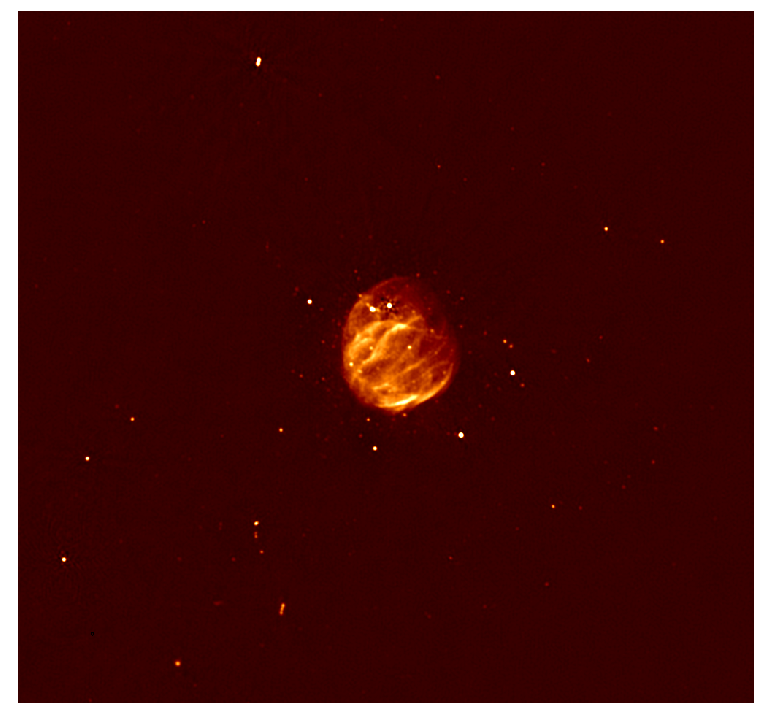
\includegraphics[width=\linewidth, trim={230px 210px 225px 200px}, clip]{./chapters/05.results/pic_G55_7.png}
		\caption{Reconstruction by NRAO.  Source:\cite{nraoG55}}
	\end{subfigure}
	\begin{subfigure}[b]{0.45\linewidth}
		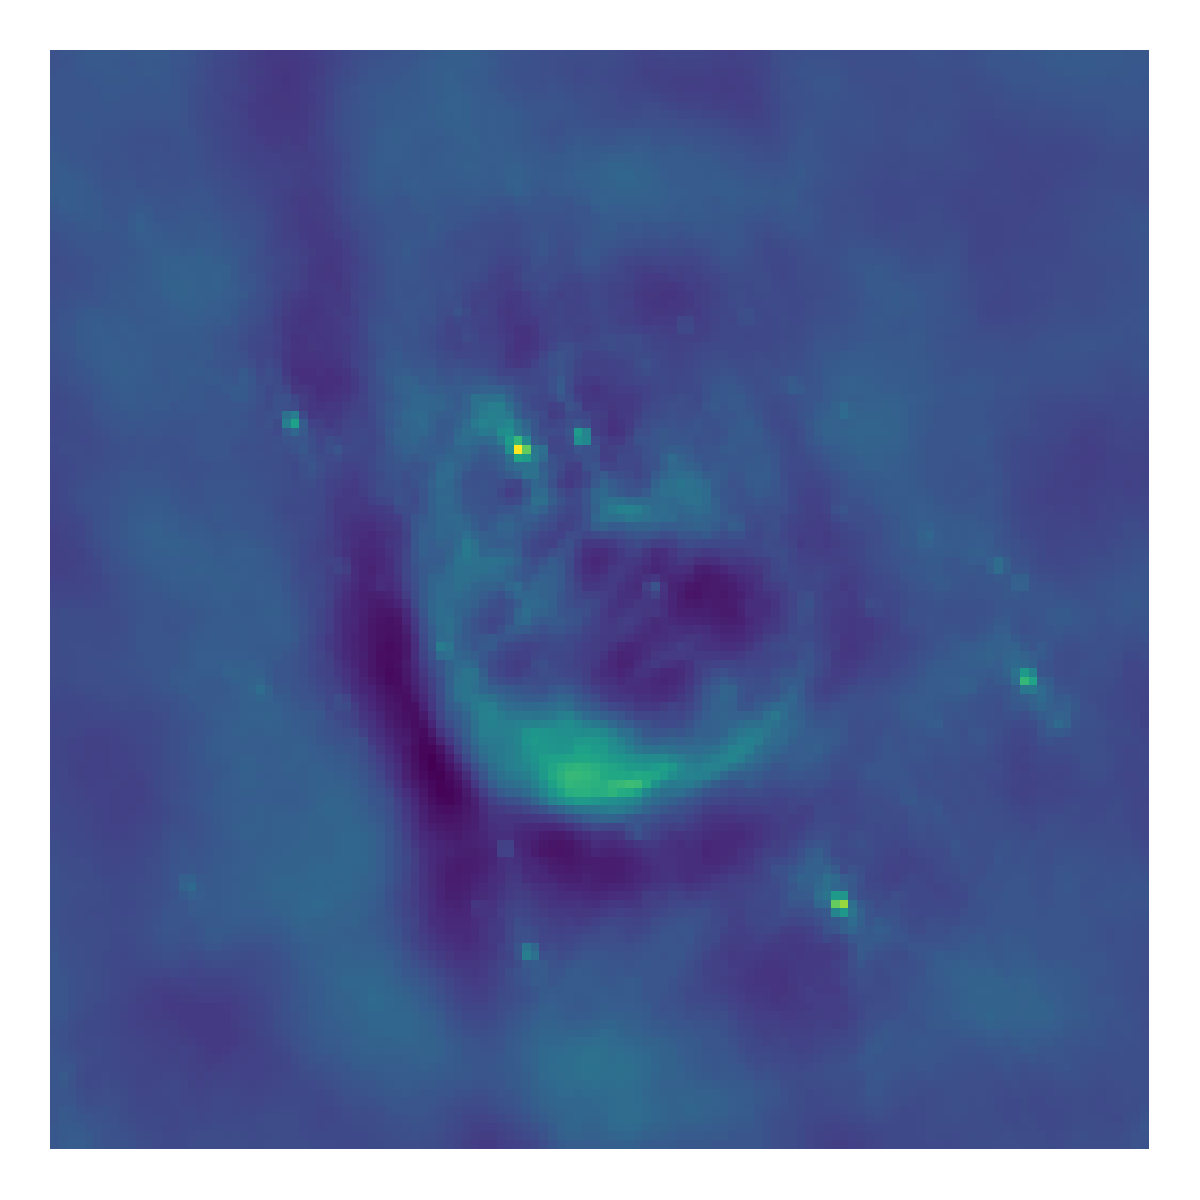
\includegraphics[width=\linewidth, trim={18px 19px 18px 18px}, clip]{./chapters/05.results/g55/raw_image.png}
		\caption{Dirty Image}
	\end{subfigure}
	\caption{SNR G55 reconstructed source observed by VLA.}
	\label{results:g55:nrao}
\end{figure}

Supernova remnant (SNR). Circle in the middle with several bright sources. The primary beam is approximately the size of the remnant, the whole image is $\approx$2 times the primary beam width.

Data from CASA imaging tutorial\cite{casaImagingGuide}. It is unknown if the data used to create \ref{results:g55:nrao} is the same as the data available for the imaging tutorial. Also the reconstruction algorithm used is unknown. Nevertheless,

Wide FoV constructs were not used, limits the dynamic range. The fainter point sources may get masked by noise.

Primary Beam is approximately the size of the remnant. The image shown here is the cutout used to compare algorithms. the full image is about twice the size of what was used in this project. [$128*128$ were used due to memory limitations.]

CLEAN algorithm, parameters were used from the imaging tutorial \cite{casaImagingGuide}
\begin{figure}[h]
	\centering
	\rotatebox{90}{\makebox{\hspace{60pt}Cleaned}}
	\begin{subfigure}[b]{0.3\linewidth}
		\begin{center}CLEAN\end{center}
		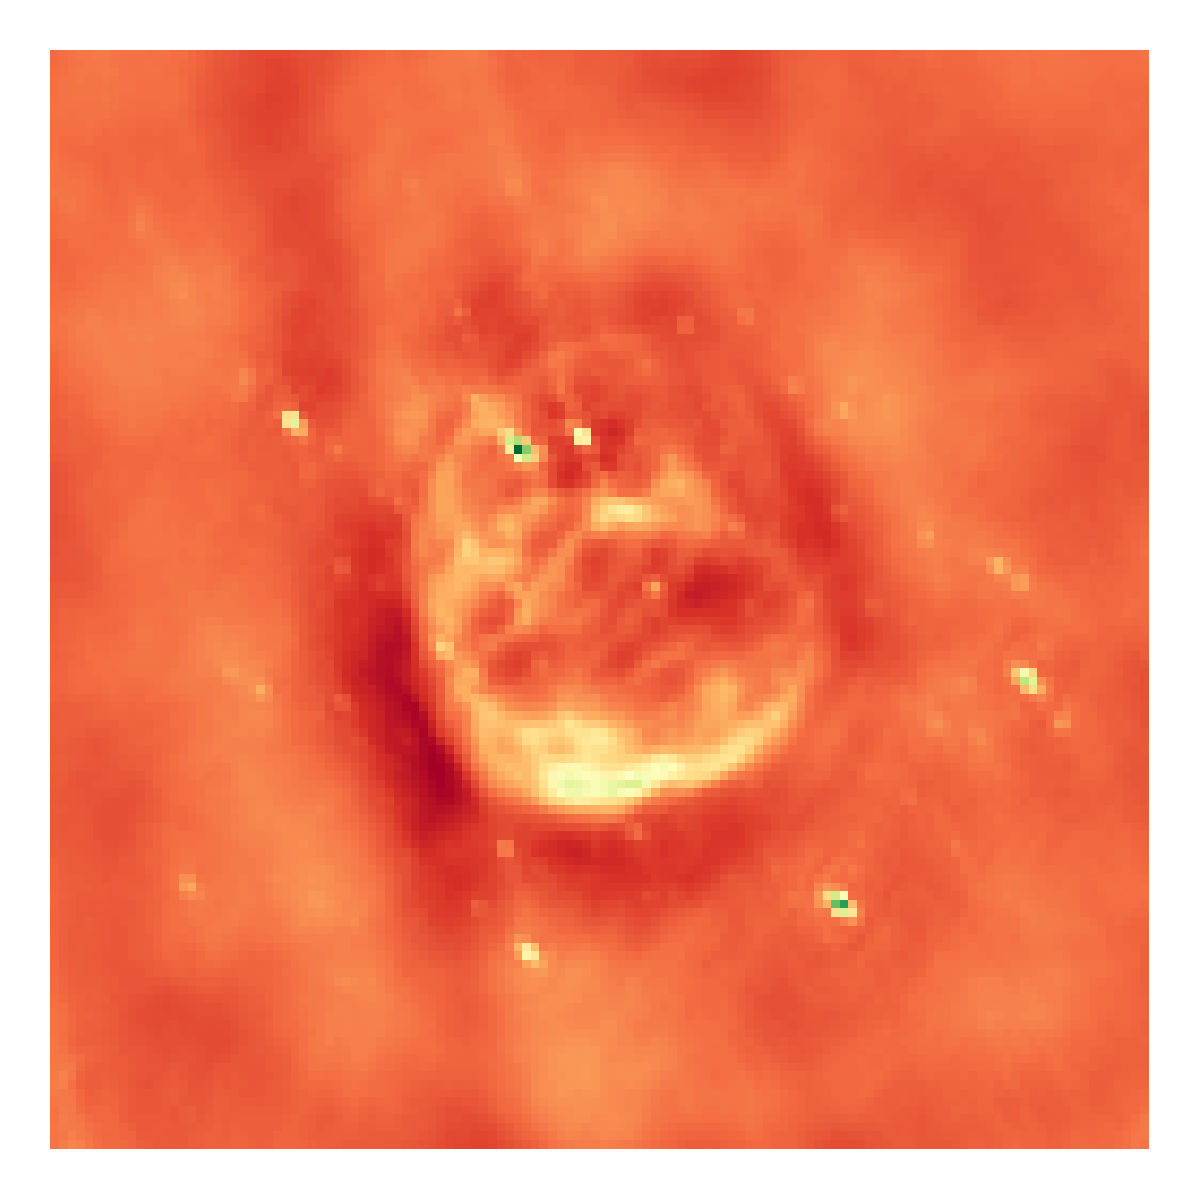
\includegraphics[width=\linewidth, trim={18px 19px 18px 18px}, clip]{./chapters/05.results/g55/clean_image.png}
	\end{subfigure}
	\begin{subfigure}[b]{0.3\linewidth}
		\begin{center}Deconvolution\end{center}
		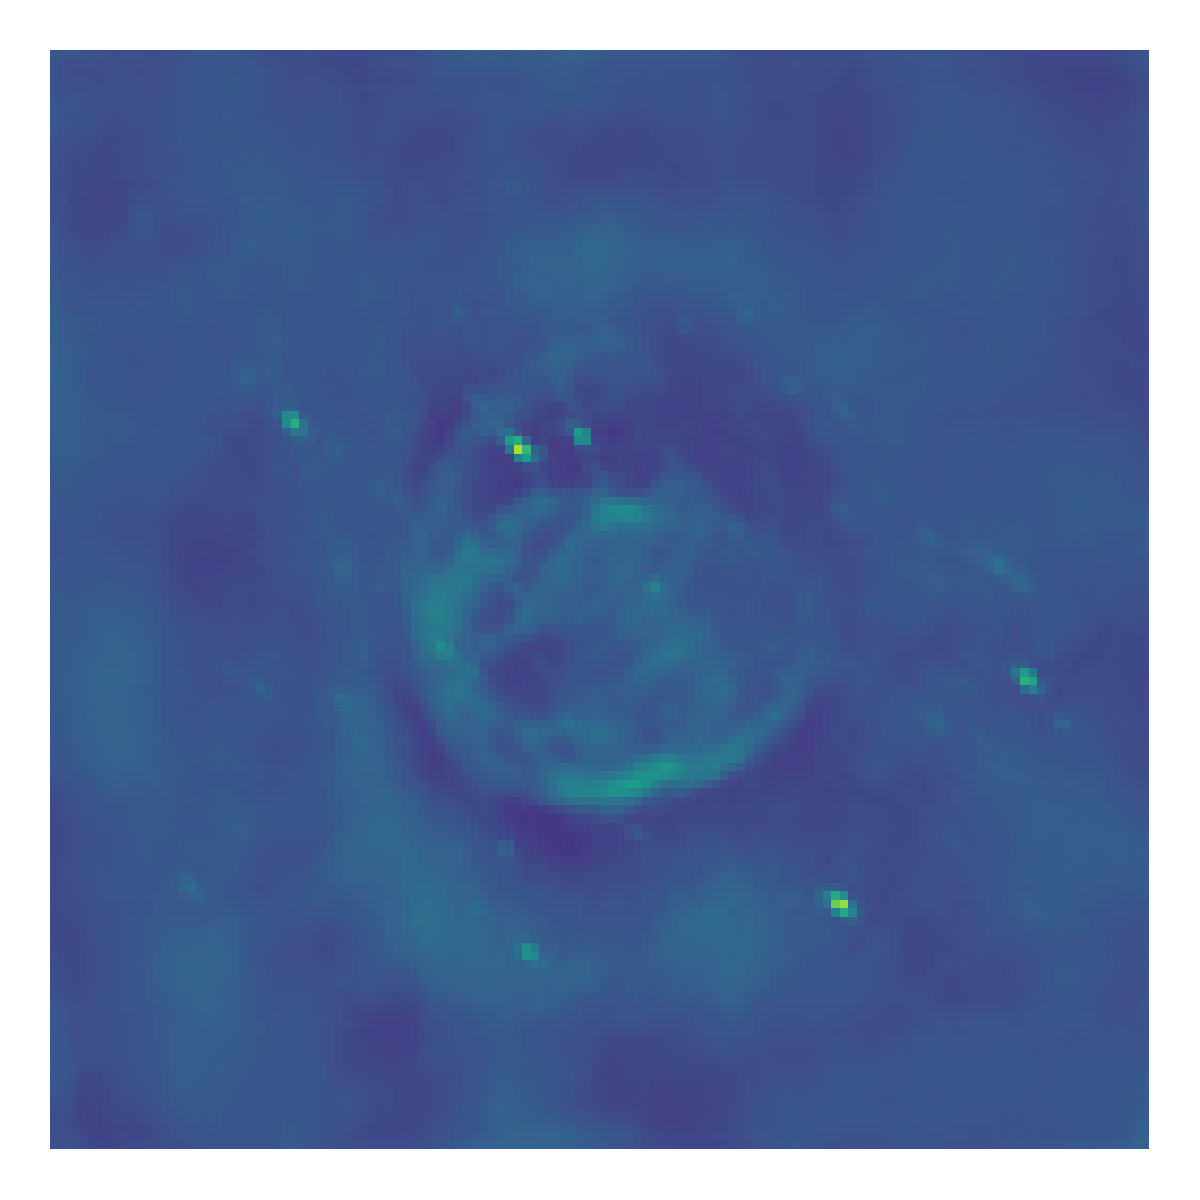
\includegraphics[width=\linewidth, trim={18px 19px 18px 18px}, clip]{./chapters/05.results/g55/positive_deconv_image.png}
	\end{subfigure}
	\begin{subfigure}[b]{0.3\linewidth}
		\begin{center}L1\end{center}
		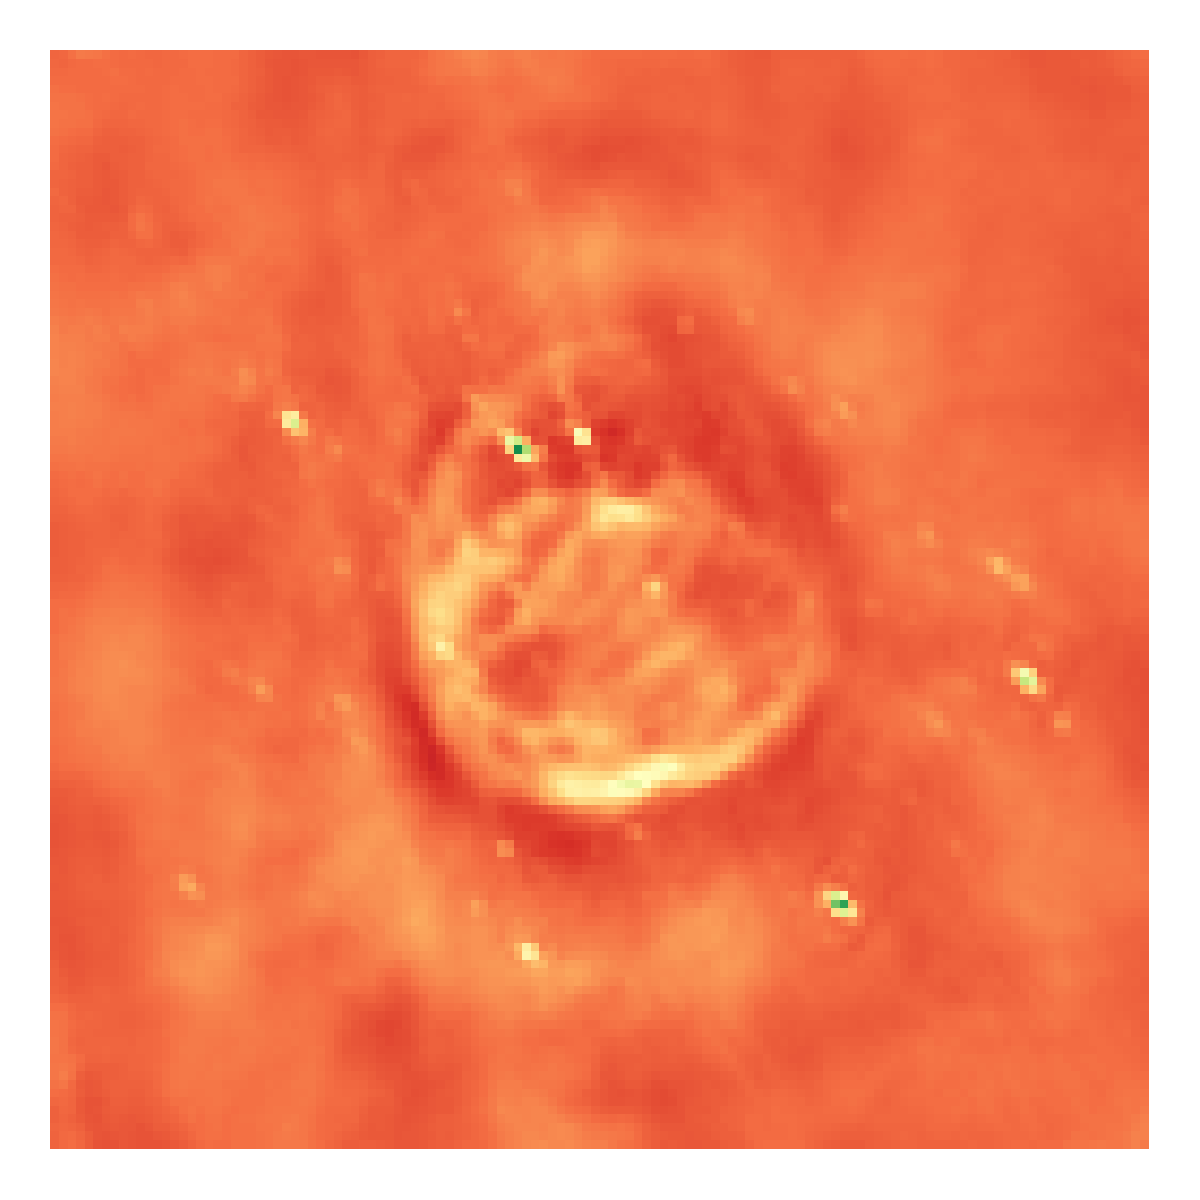
\includegraphics[width=\linewidth, trim={18px 19px 18px 18px}, clip]{./chapters/05.results/g55/L1_image.png}
	\end{subfigure}

	\rotatebox{90}{\makebox{\hspace{60pt}Model}}
	\begin{subfigure}[b]{0.3\linewidth}
		
\includegraphics[width=\linewidth, trim={18px 19px 18px 18px}, clip]{./chapters/05.results/g55/clean_model.png}
	\end{subfigure}
	\begin{subfigure}[b]{0.3\linewidth}
		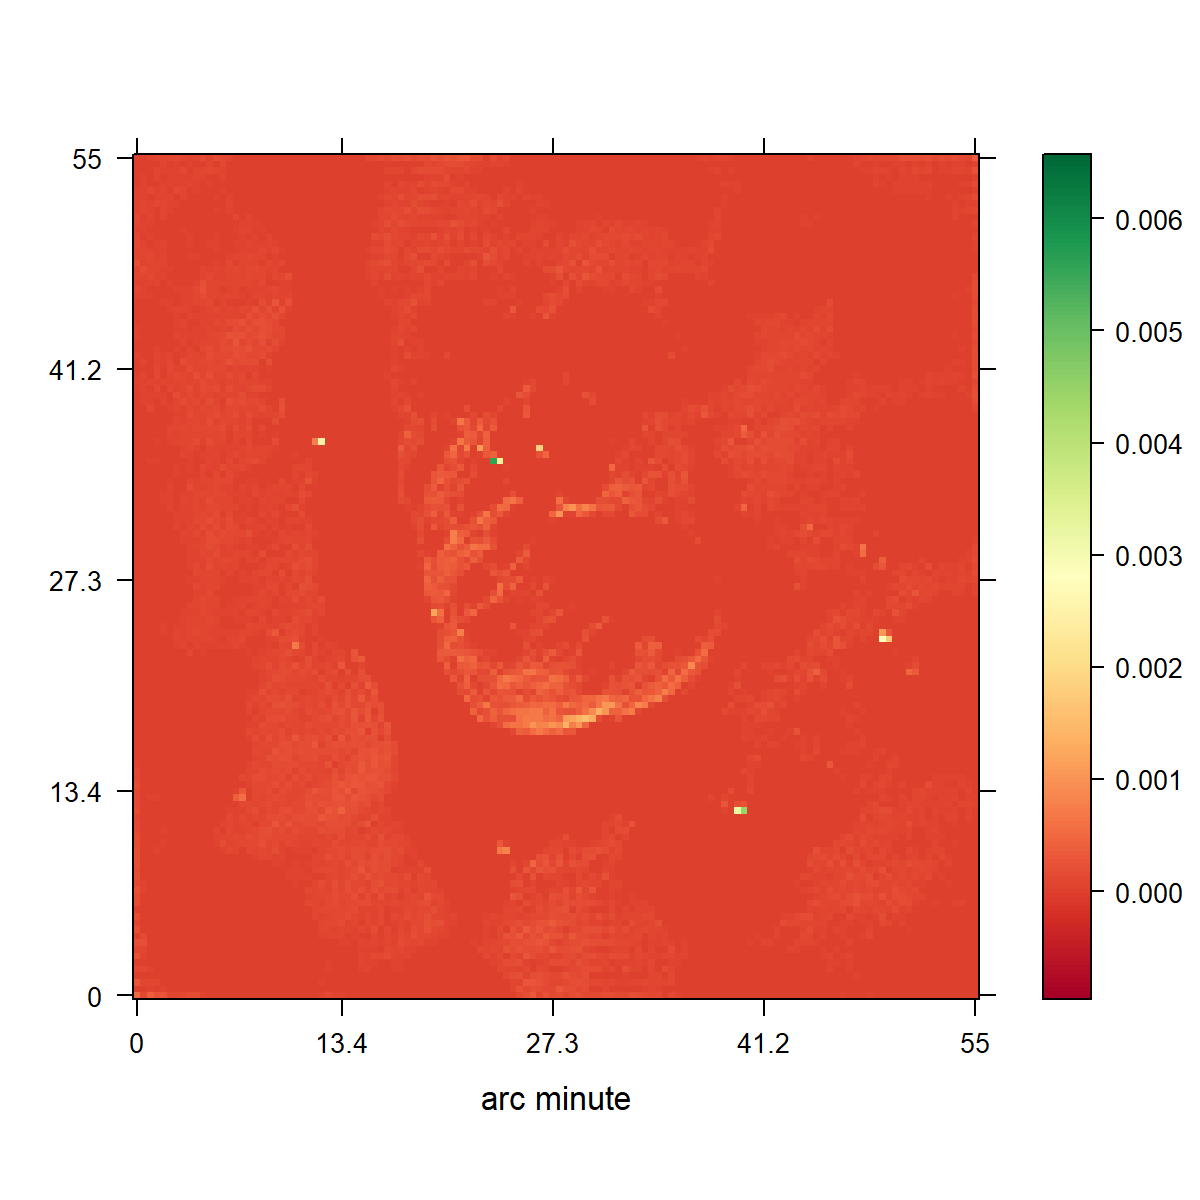
\includegraphics[width=\linewidth, trim={18px 19px 18px 18px}, clip]{./chapters/05.results/g55/positive_deconv_model.png}
	\end{subfigure}
	\begin{subfigure}[b]{0.3\linewidth}
		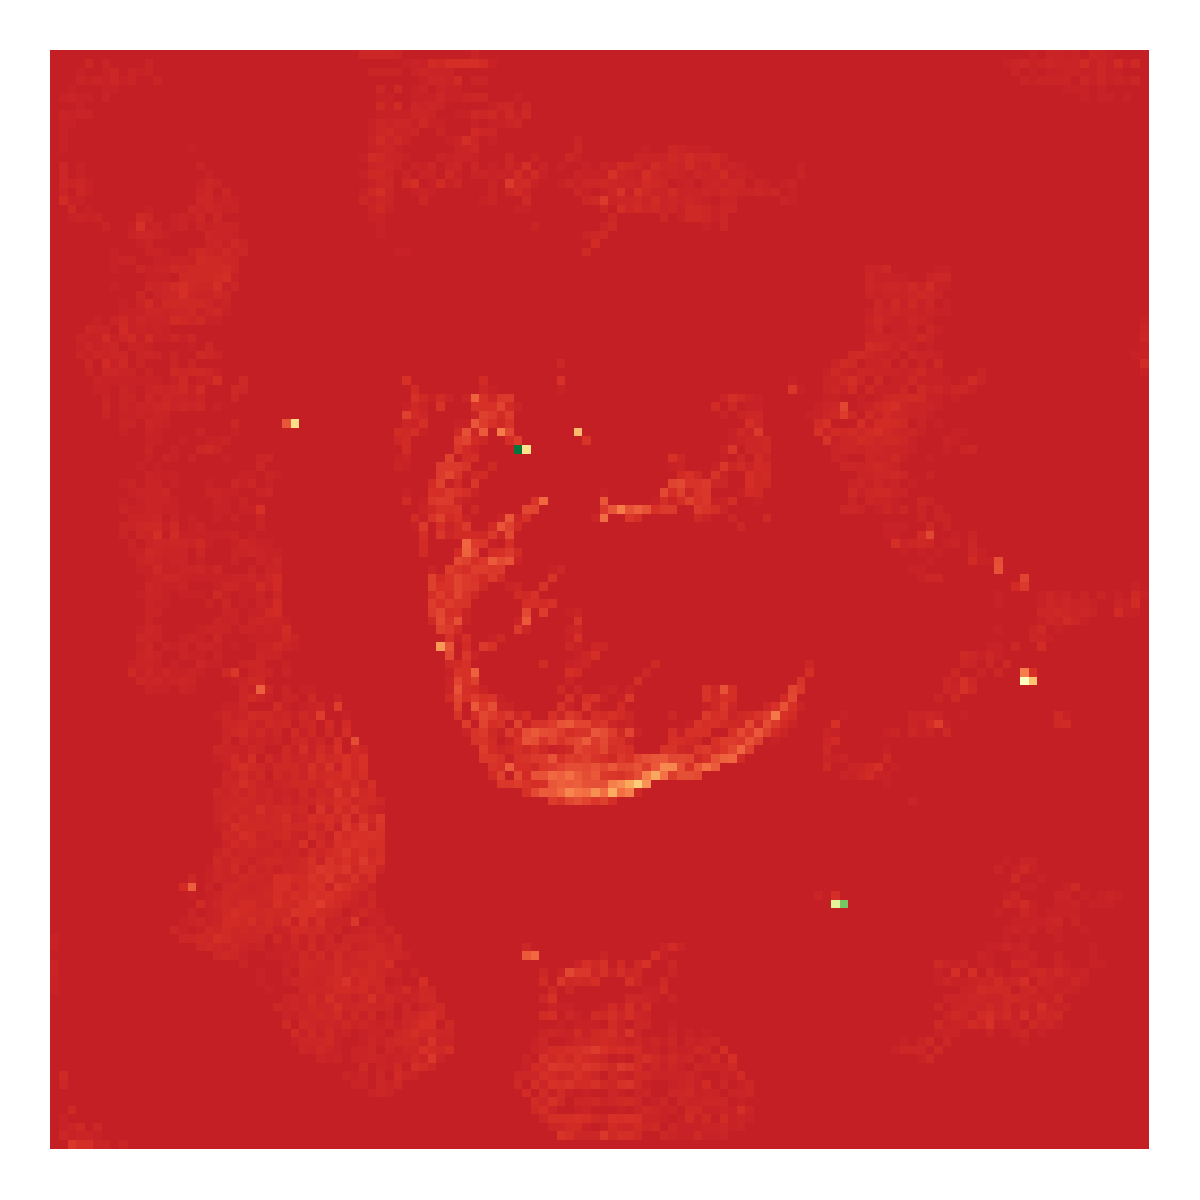
\includegraphics[width=\linewidth, trim={18px 19px 18px 18px}, clip]{./chapters/05.results/g55/L1_model.png}
	\end{subfigure}

	\rotatebox{90}{\makebox{\hspace{60pt}Residuals}}
	\begin{subfigure}[b]{0.3\linewidth}
		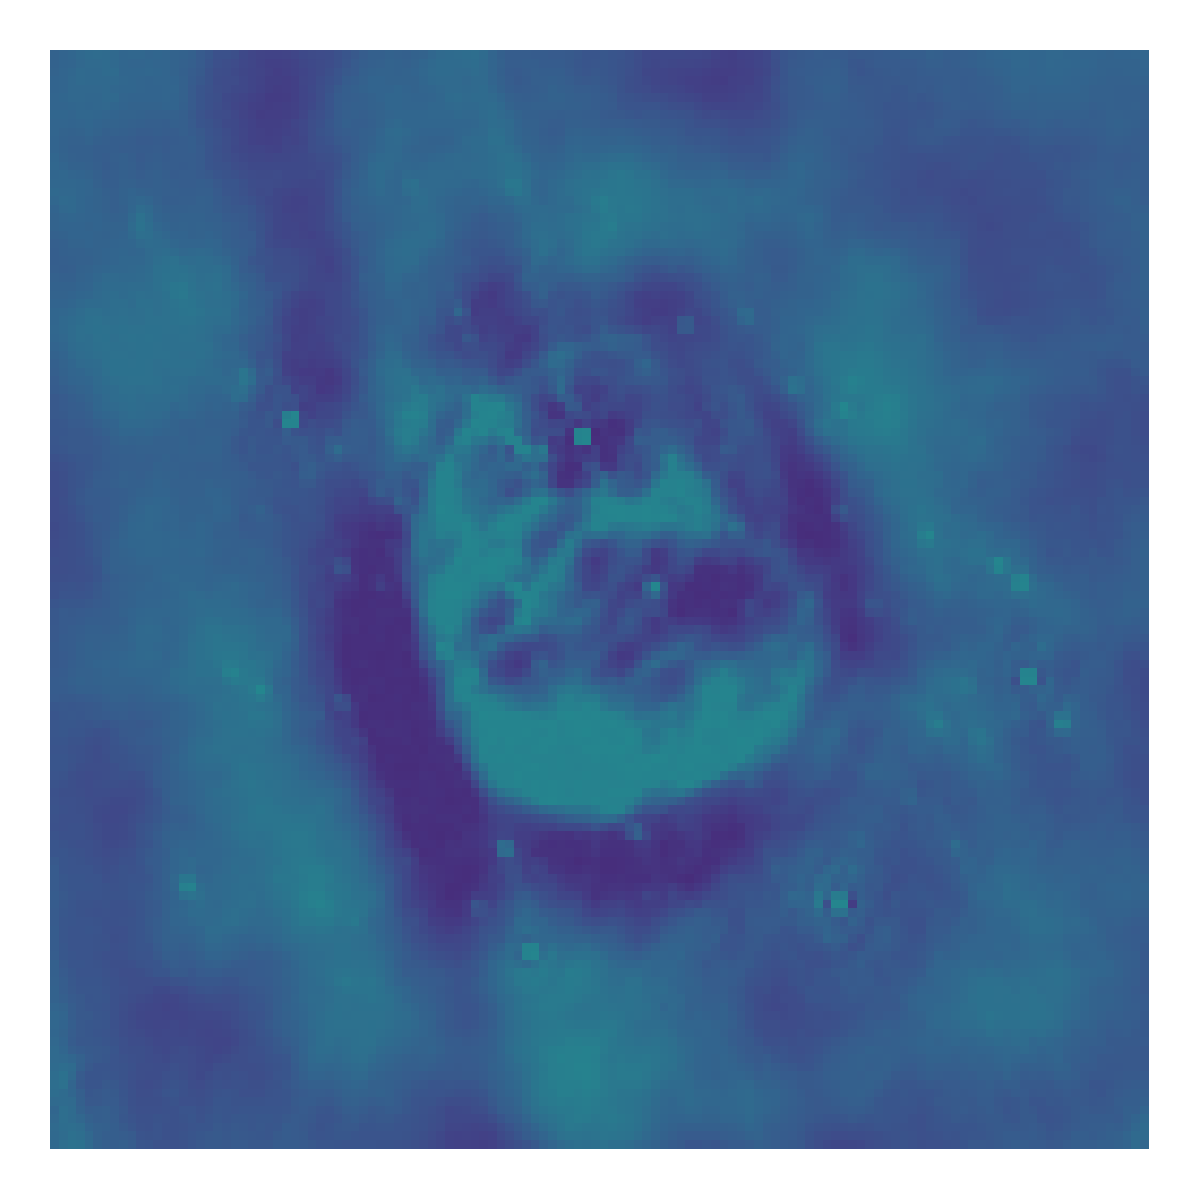
\includegraphics[width=\linewidth, trim={18px 19px 18px 18px}, clip]{./chapters/05.results/g55/clean_residual.png}
		\begin{center}RMS: 0.03957\end{center}
	\end{subfigure}
	\begin{subfigure}[b]{0.3\linewidth}
		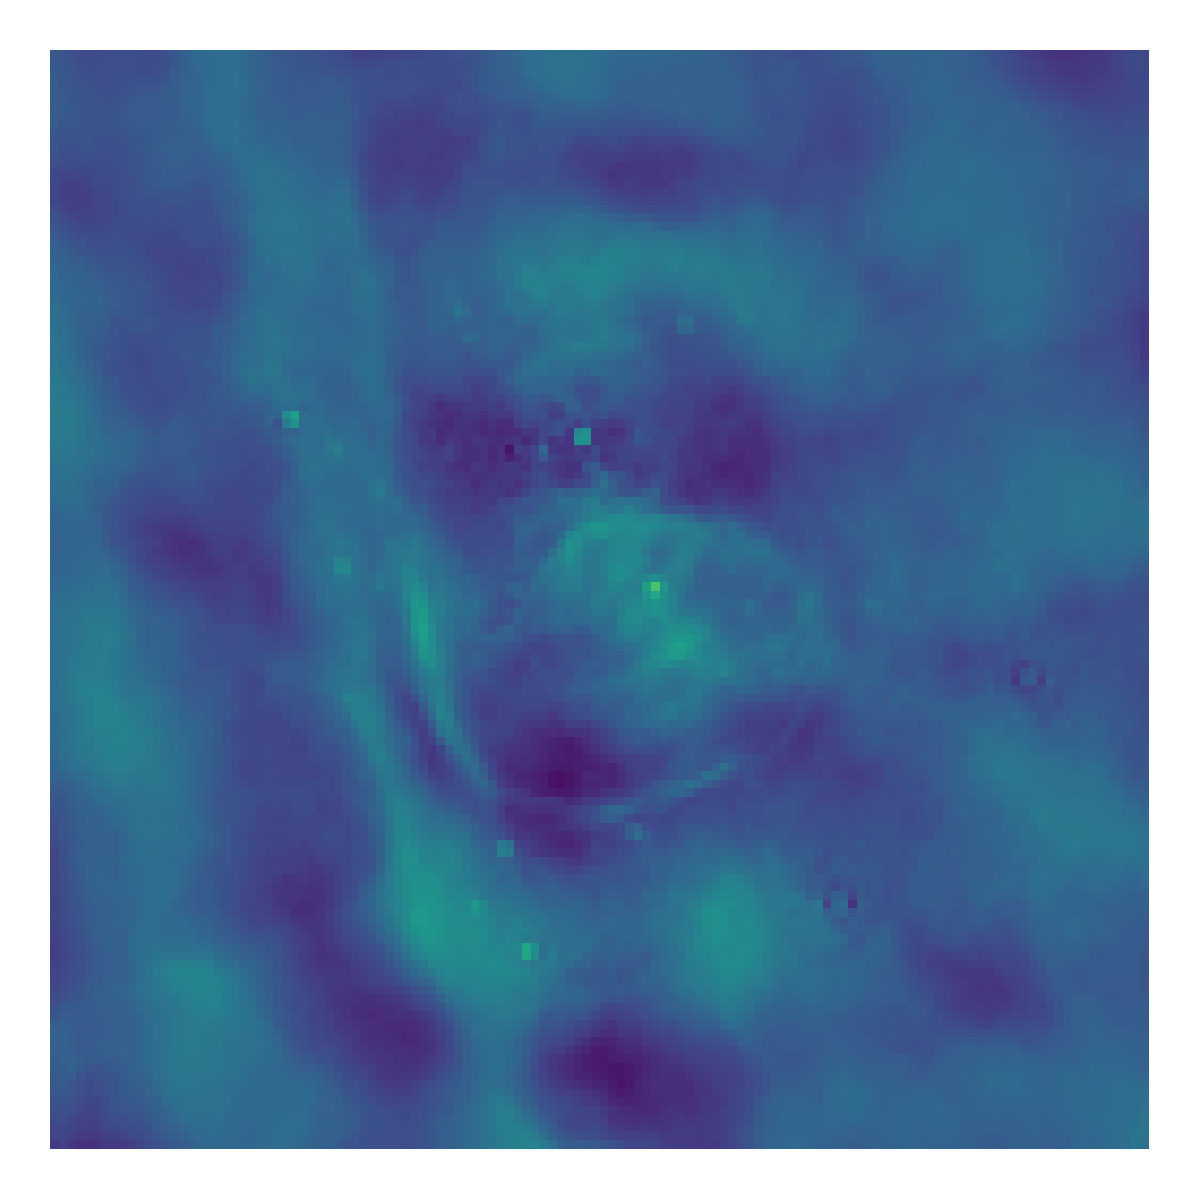
\includegraphics[width=\linewidth, trim={18px 19px 18px 18px}, clip]{./chapters/05.results/g55/positive_deconv_residual.png}
		\begin{center}RMS: 0.04406\end{center}
	\end{subfigure}
	\begin{subfigure}[b]{0.3\linewidth}
		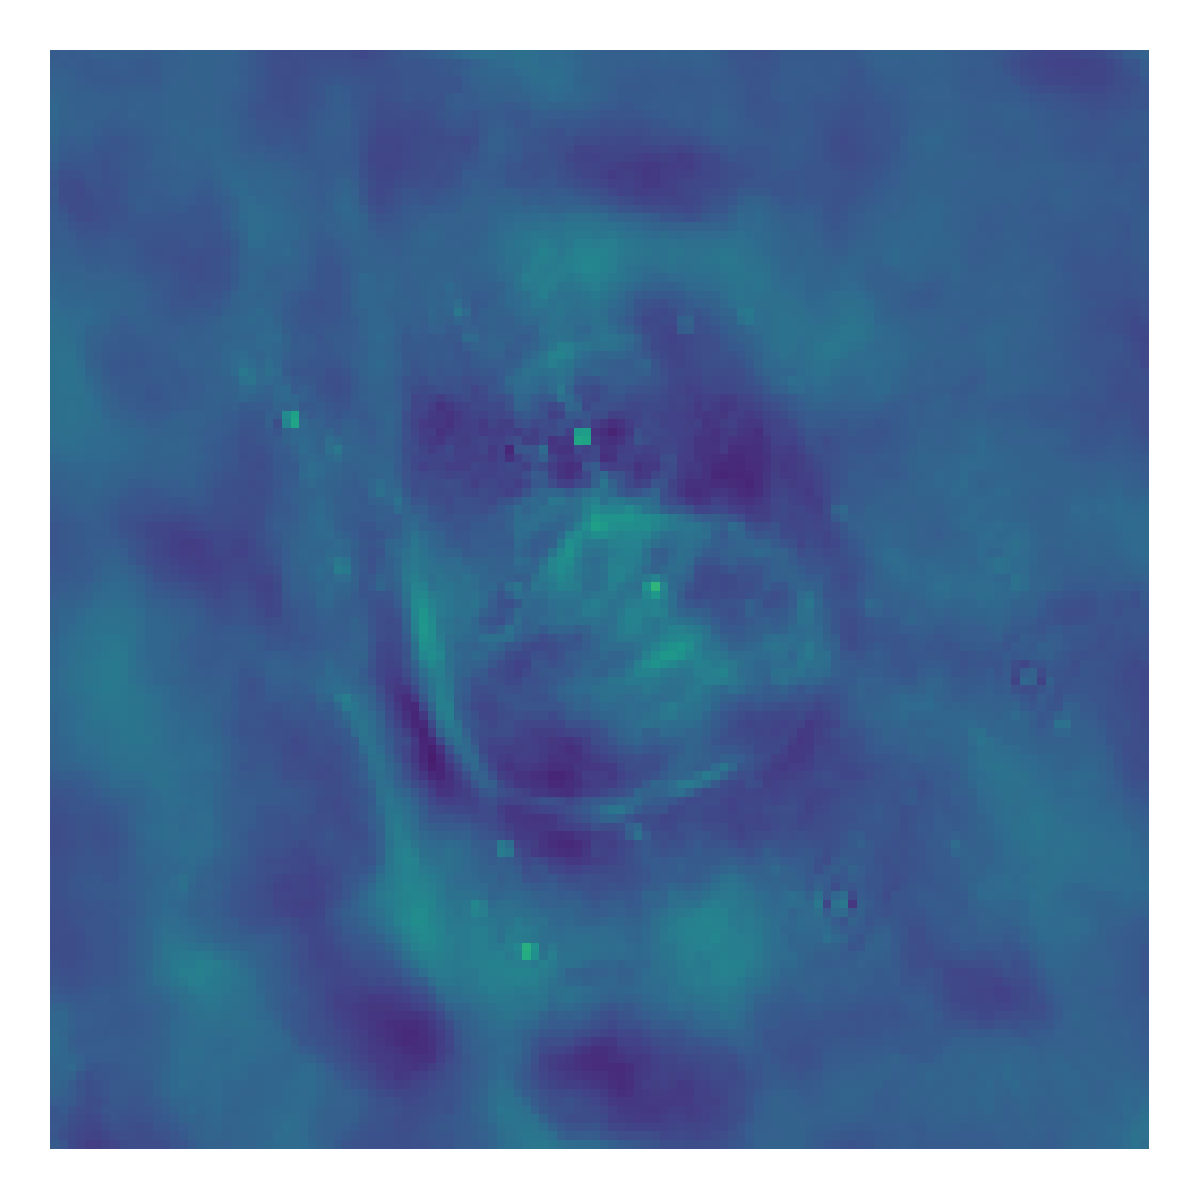
\includegraphics[width=\linewidth, trim={18px 19px 18px 18px}, clip]{./chapters/05.results/g55/L1_residual.png}
		\begin{center}RMS: 0.03460\end{center}
	\end{subfigure}
	\caption{Simple priors compared with tclean}
\end{figure}




\begin{figure}[h]
	\centering
	\rotatebox{90}{\makebox{\hspace{60pt}Cleaned}}
	\begin{subfigure}[b]{0.3\linewidth}
		\begin{center}CLEAN\end{center}
		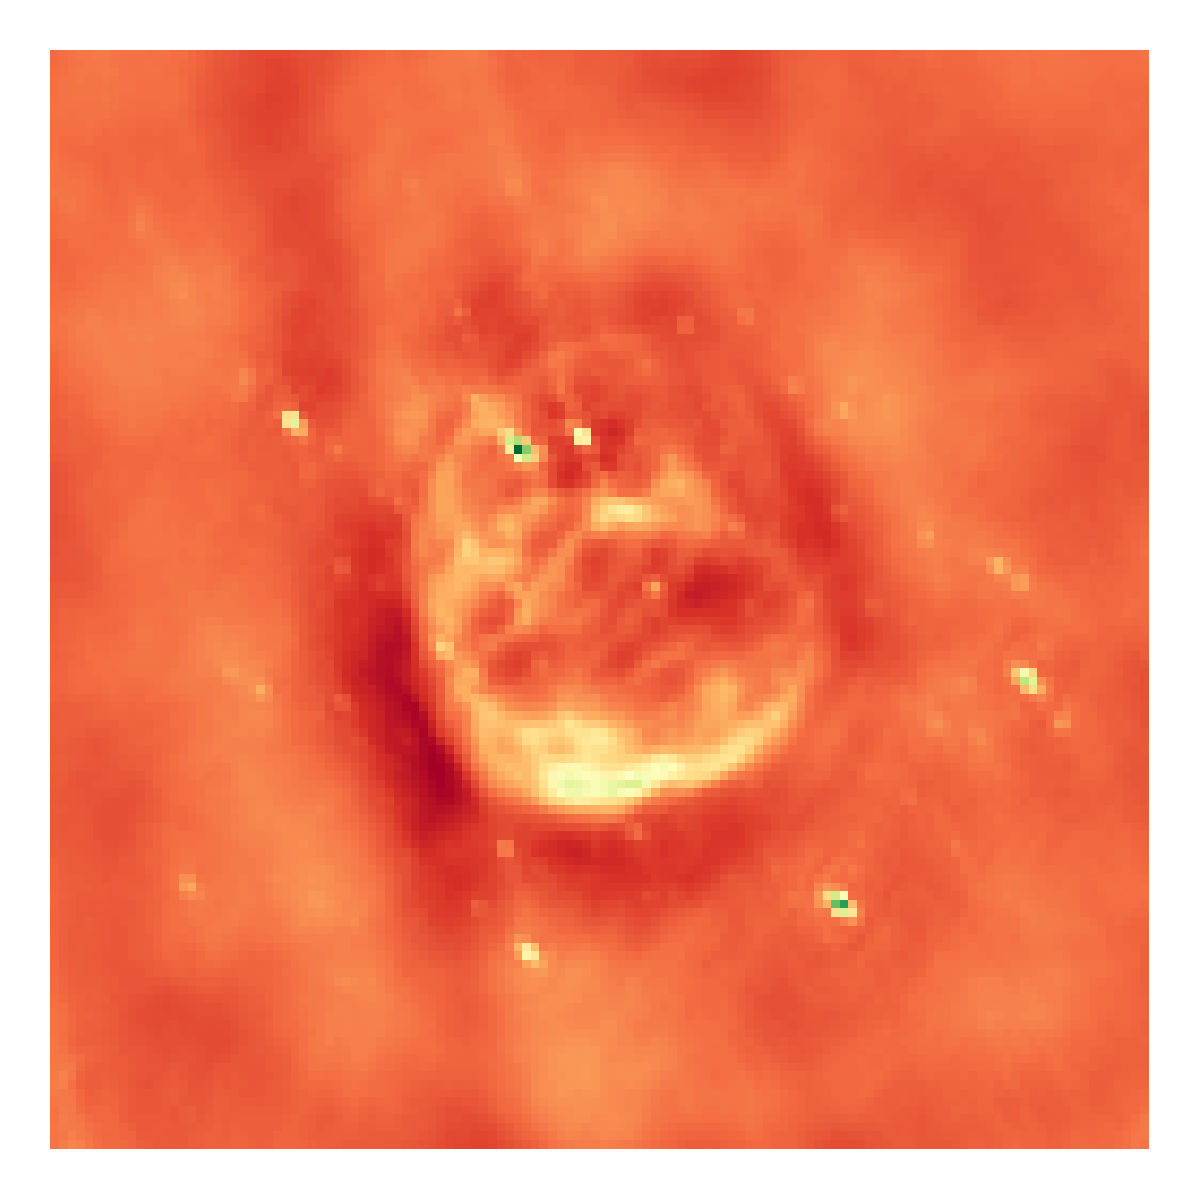
\includegraphics[width=\linewidth, trim={18px 19px 18px 18px}, clip]{./chapters/05.results/g55/clean_image.png}
	\end{subfigure}
	\begin{subfigure}[b]{0.3\linewidth}
		\begin{center}L2\end{center}
		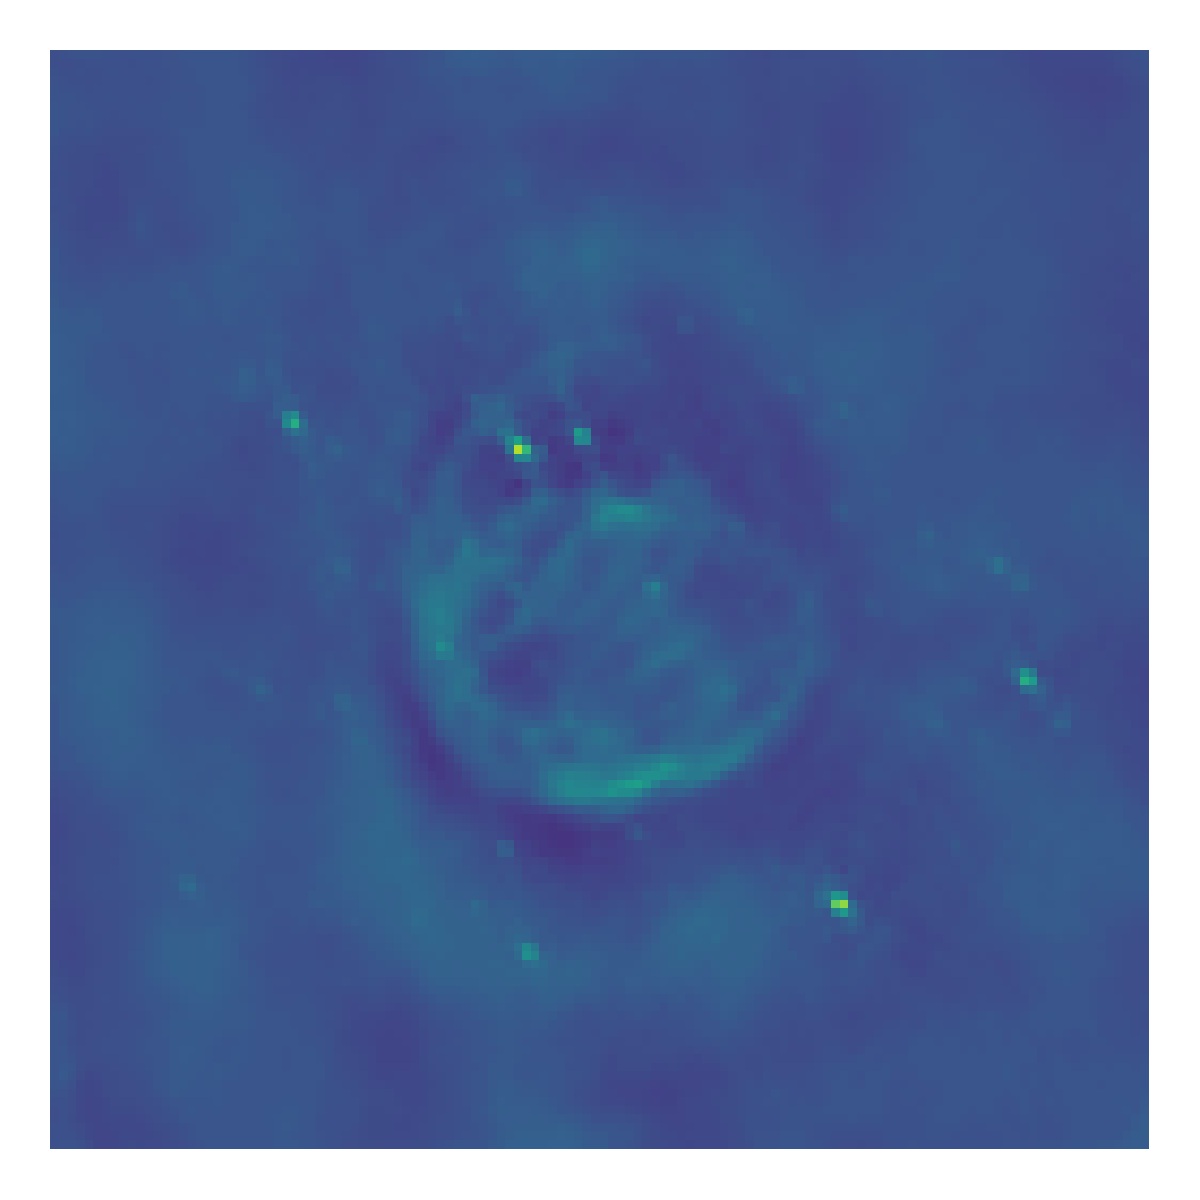
\includegraphics[width=\linewidth, trim={18px 19px 18px 18px}, clip]{./chapters/05.results/g55/L2_image.png}
	\end{subfigure}
	\begin{subfigure}[b]{0.3\linewidth}
		\begin{center}Total Variation\end{center}
		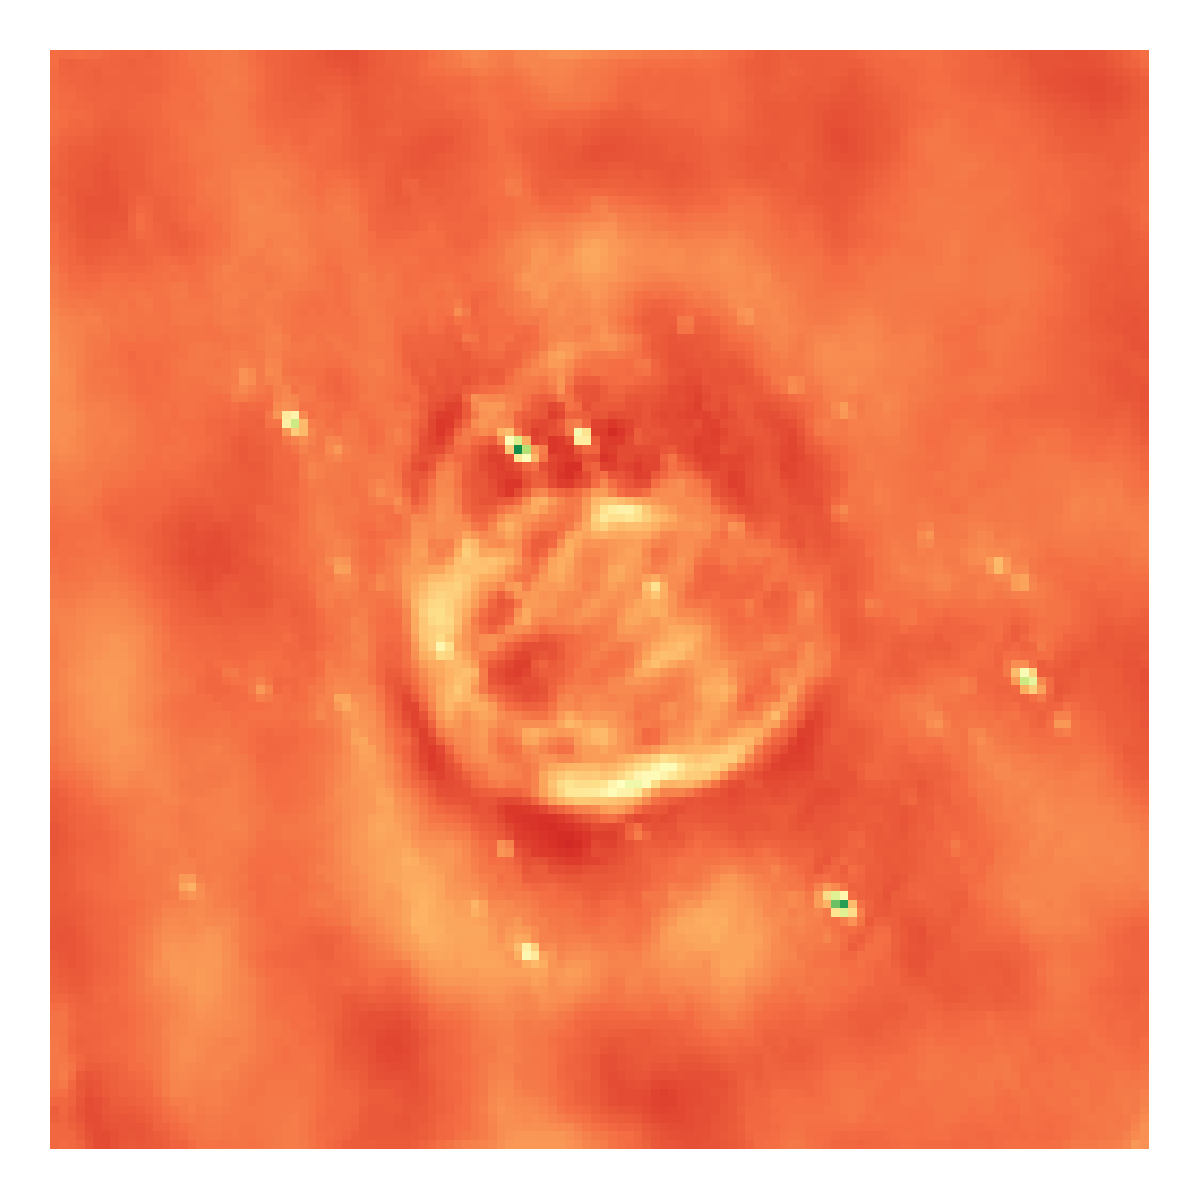
\includegraphics[width=\linewidth, trim={18px 19px 18px 18px}, clip]{./chapters/05.results/g55/TV_image.png}
	\end{subfigure}

	\rotatebox{90}{\makebox{\hspace{60pt}Model}}
	\begin{subfigure}[b]{0.3\linewidth}
		
\includegraphics[width=\linewidth, trim={18px 19px 18px 18px}, clip]{./chapters/05.results/g55/clean_model.png}
	\end{subfigure}
	\begin{subfigure}[b]{0.3\linewidth}
		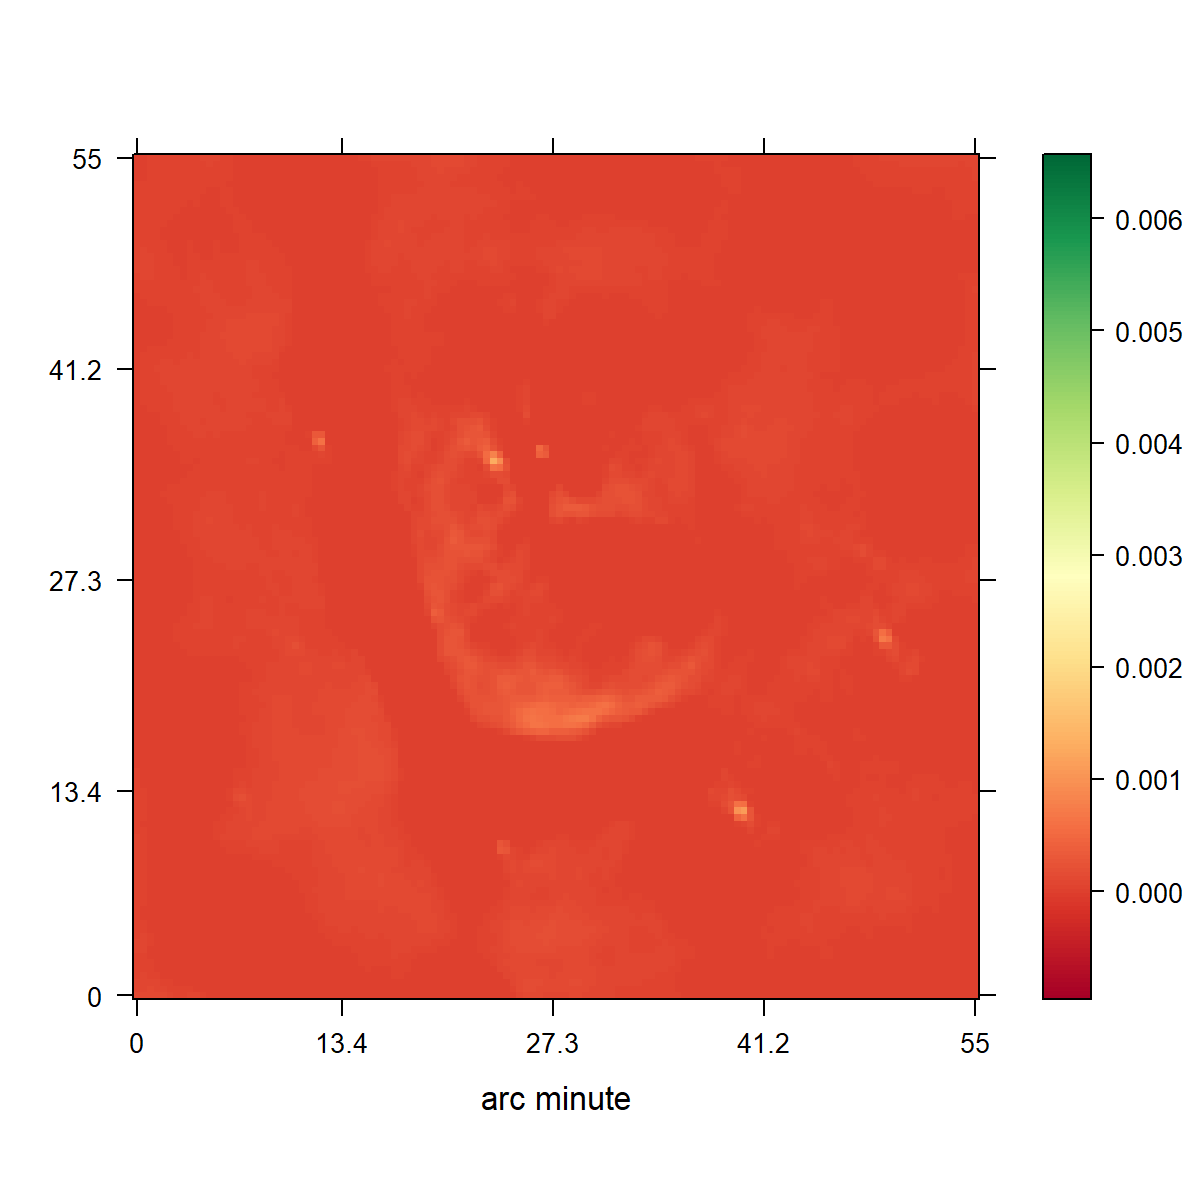
\includegraphics[width=\linewidth, trim={18px 19px 18px 18px}, clip]{./chapters/05.results/g55/L2_model.png}
	\end{subfigure}
	\begin{subfigure}[b]{0.3\linewidth}
		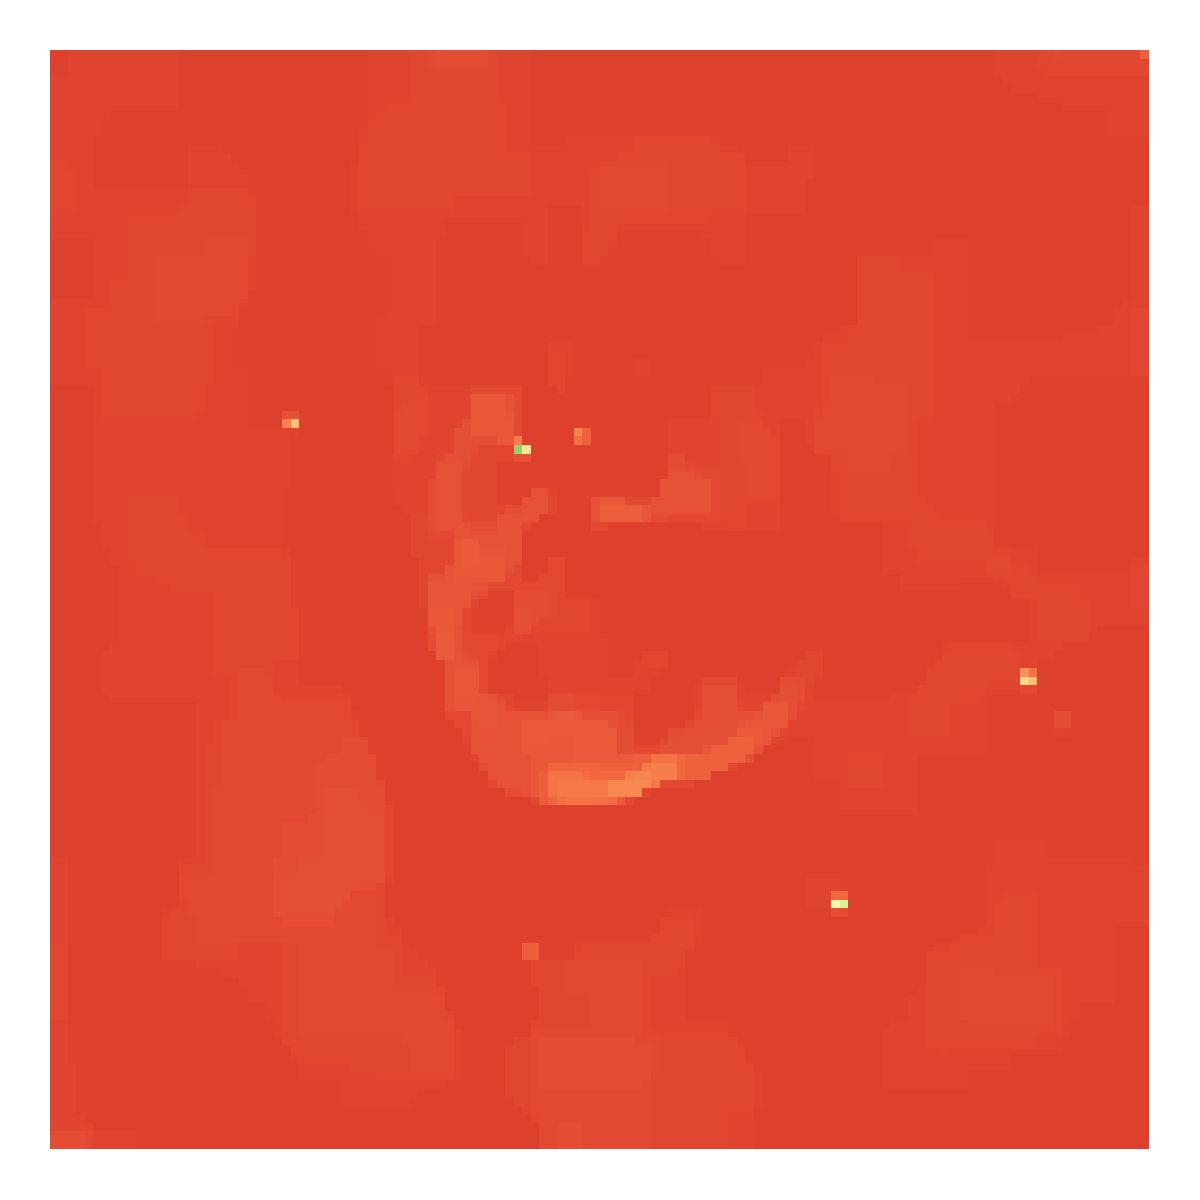
\includegraphics[width=\linewidth, trim={18px 19px 18px 18px}, clip]{./chapters/05.results/g55/TV_model.png}
	\end{subfigure}
	
	\rotatebox{90}{\makebox{\hspace{60pt}Residuals}}
	\begin{subfigure}[b]{0.3\linewidth}
		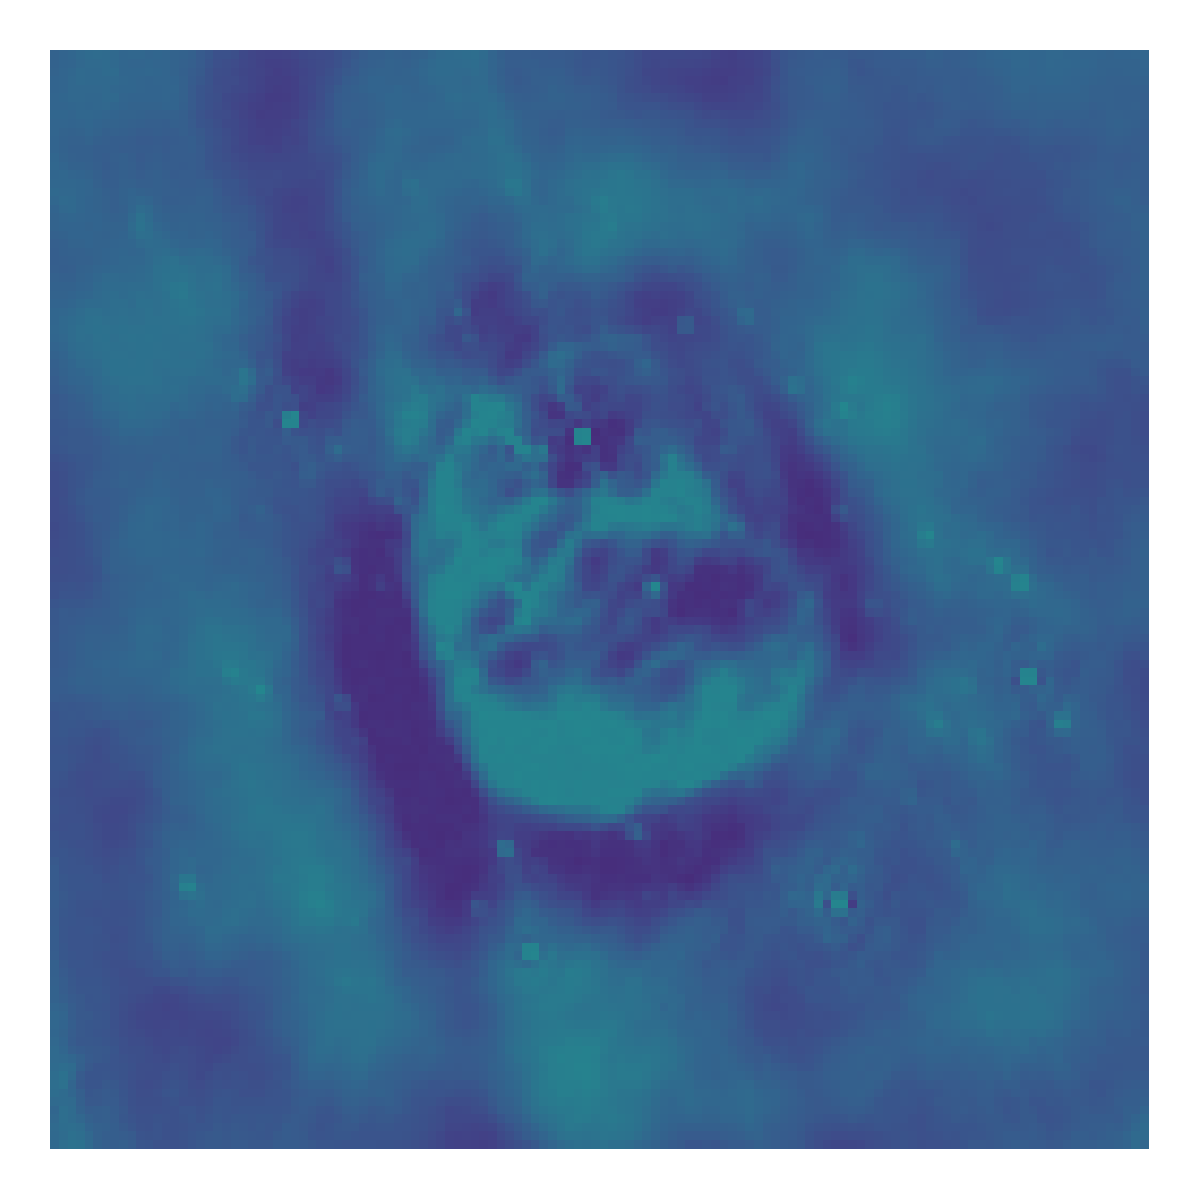
\includegraphics[width=\linewidth, trim={18px 19px 18px 18px}, clip]{./chapters/05.results/g55/clean_residual.png}
	\end{subfigure}
	\begin{subfigure}[b]{0.3\linewidth}
		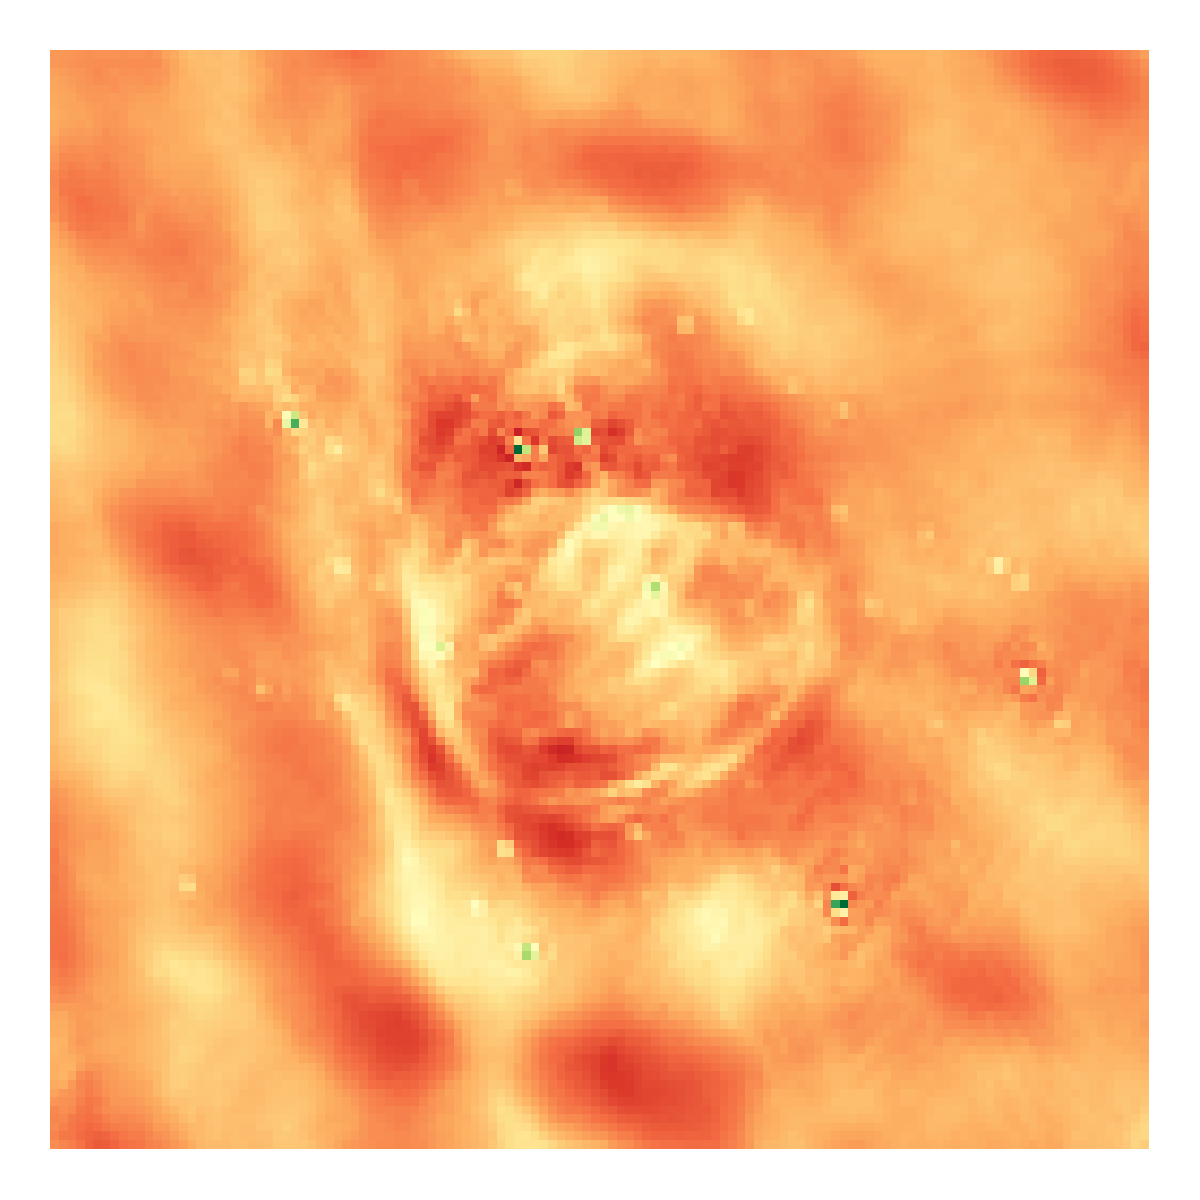
\includegraphics[width=\linewidth, trim={18px 19px 18px 18px}, clip]{./chapters/05.results/g55/L2_residual.png}
	\end{subfigure}
	\begin{subfigure}[b]{0.3\linewidth}
		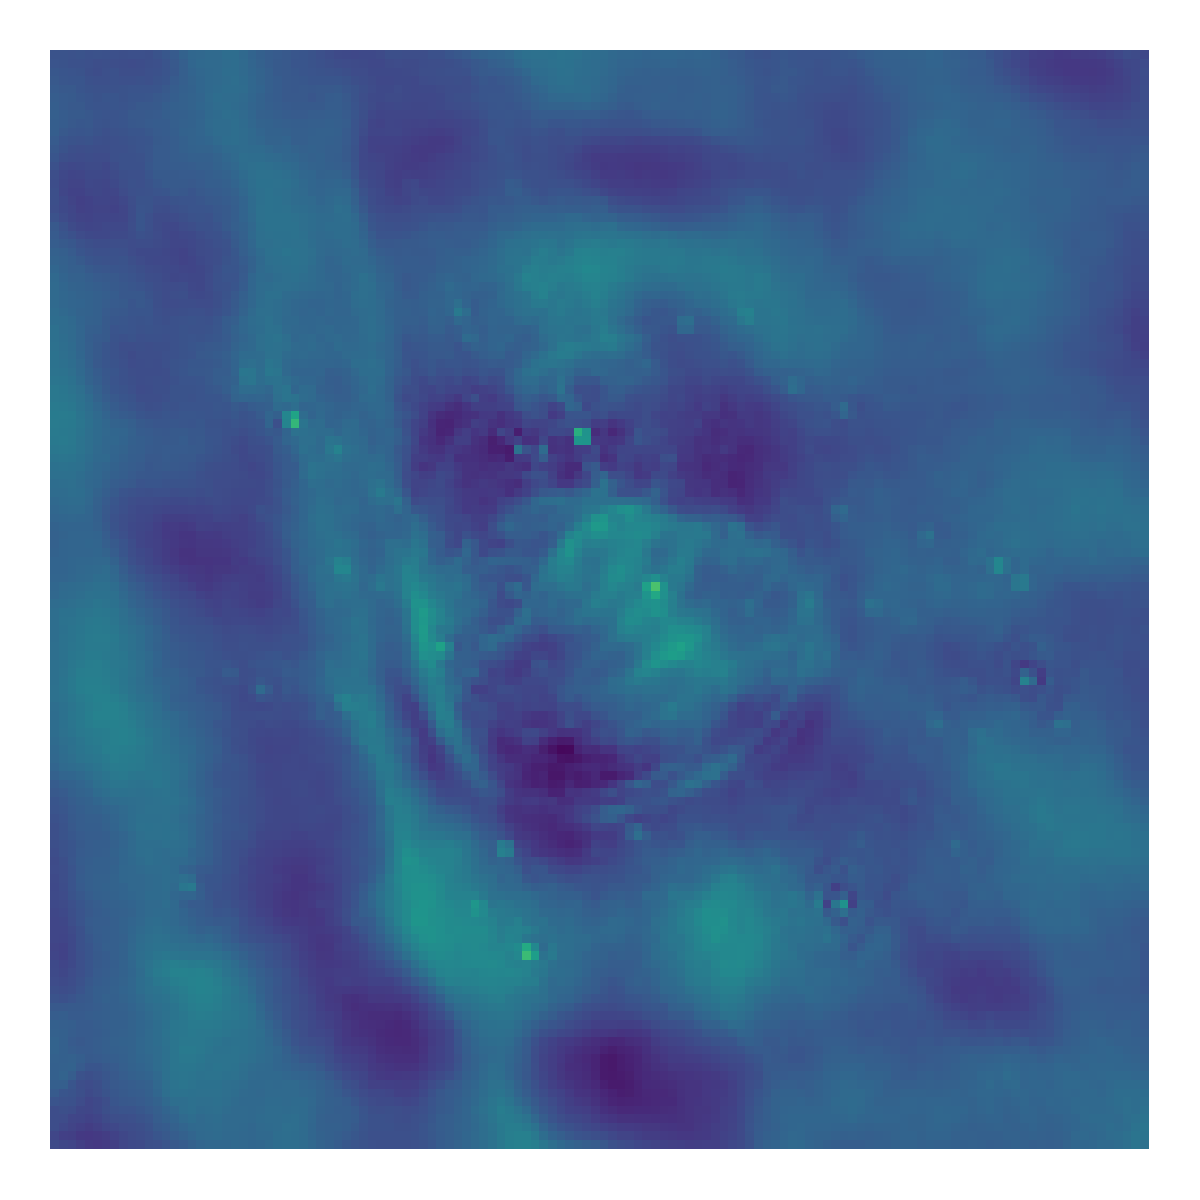
\includegraphics[width=\linewidth, trim={18px 19px 18px 18px}, clip]{./chapters/05.results/g55/TV_residual.png}
	\end{subfigure}
\end{figure}

L2 has some really high peaks in the residuals

Total Variation Prior has trouble with point sources in extended emissions

\begin{figure}[h]
	\centering
	\rotatebox{90}{\makebox{\hspace{60pt}Cleaned}}
	\begin{subfigure}[b]{0.3\linewidth}
		\begin{center}CLEAN\end{center}
		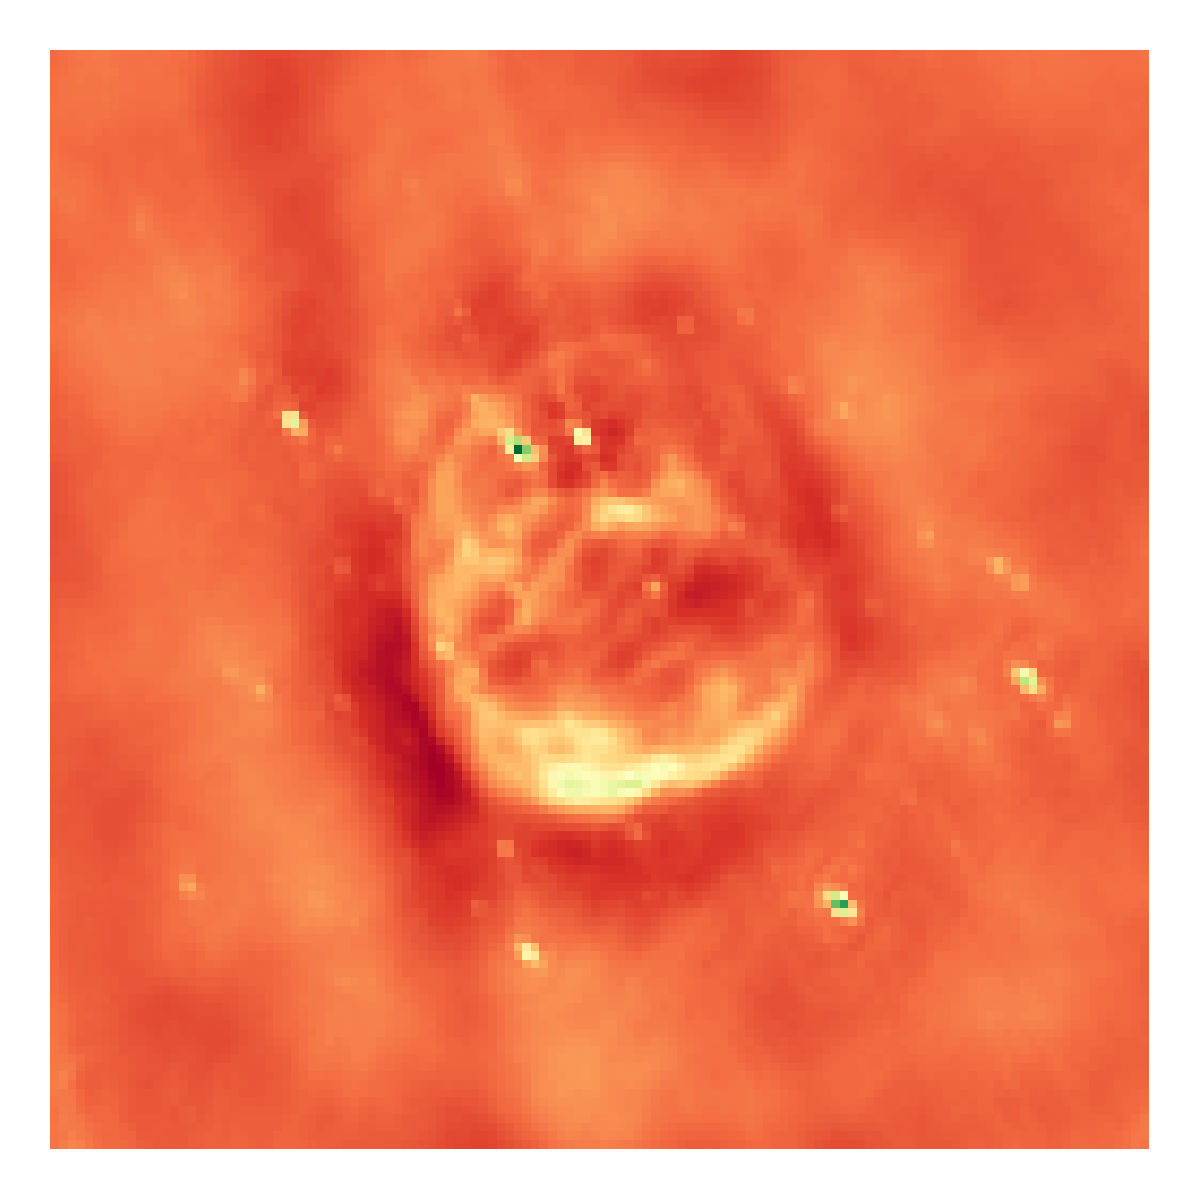
\includegraphics[width=\linewidth, trim={18px 19px 18px 18px}, clip]{./chapters/05.results/g55/clean_image.png}
	\end{subfigure}
	\begin{subfigure}[b]{0.3\linewidth}
		\begin{center}Starlets 1\end{center}
		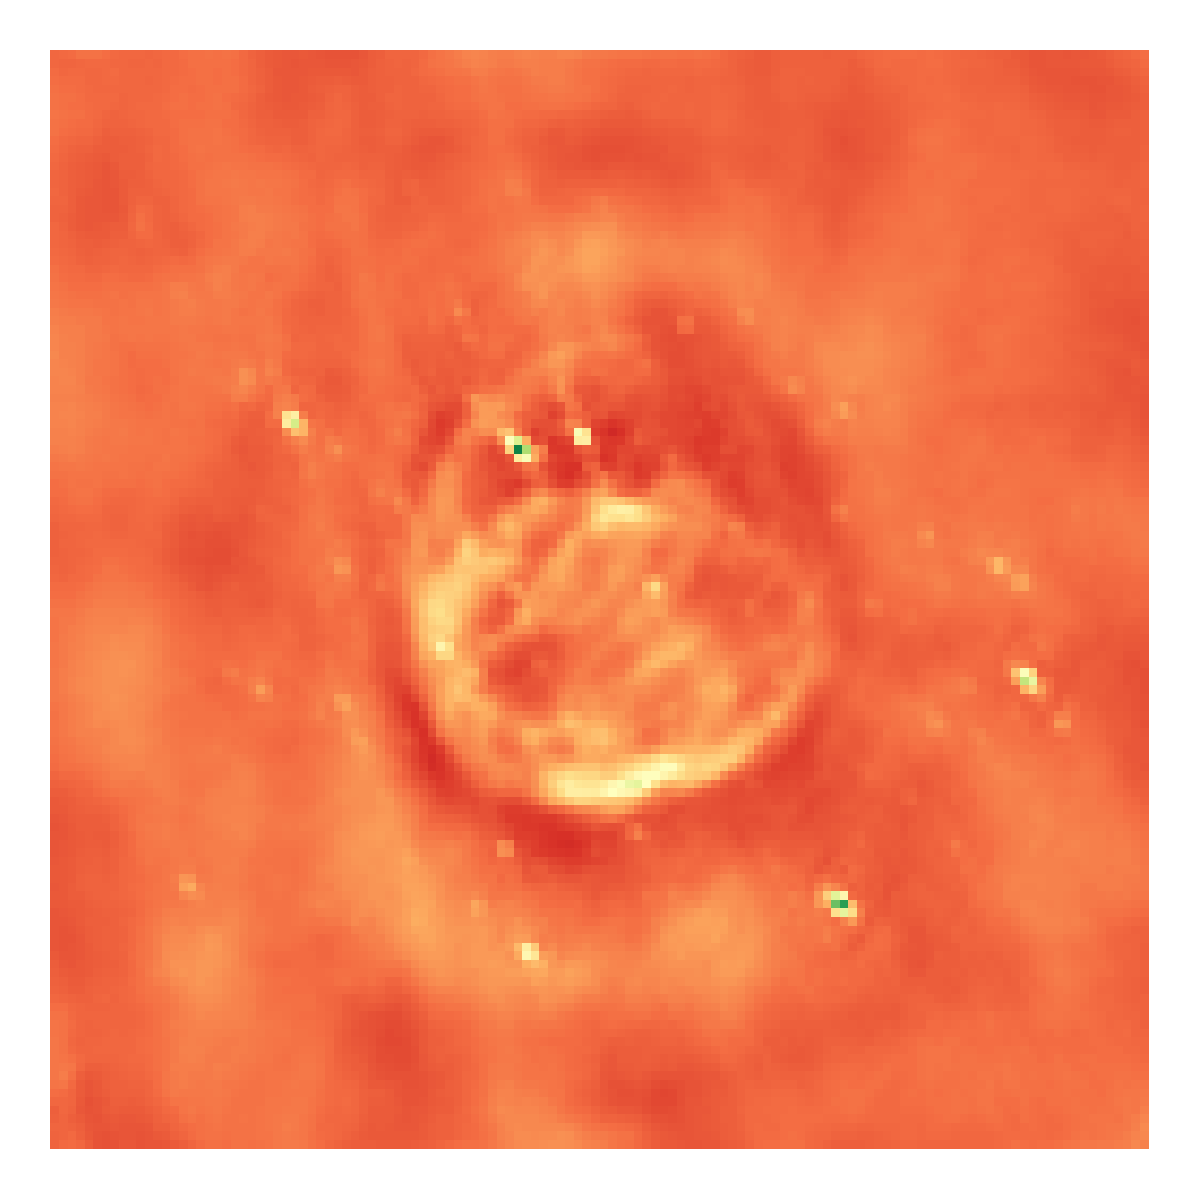
\includegraphics[width=\linewidth, trim={18px 19px 18px 18px}, clip]{./chapters/05.results/g55/starlets1_image.png}
	\end{subfigure}
	\begin{subfigure}[b]{0.3\linewidth}
		\begin{center}Starlets 3\end{center}
		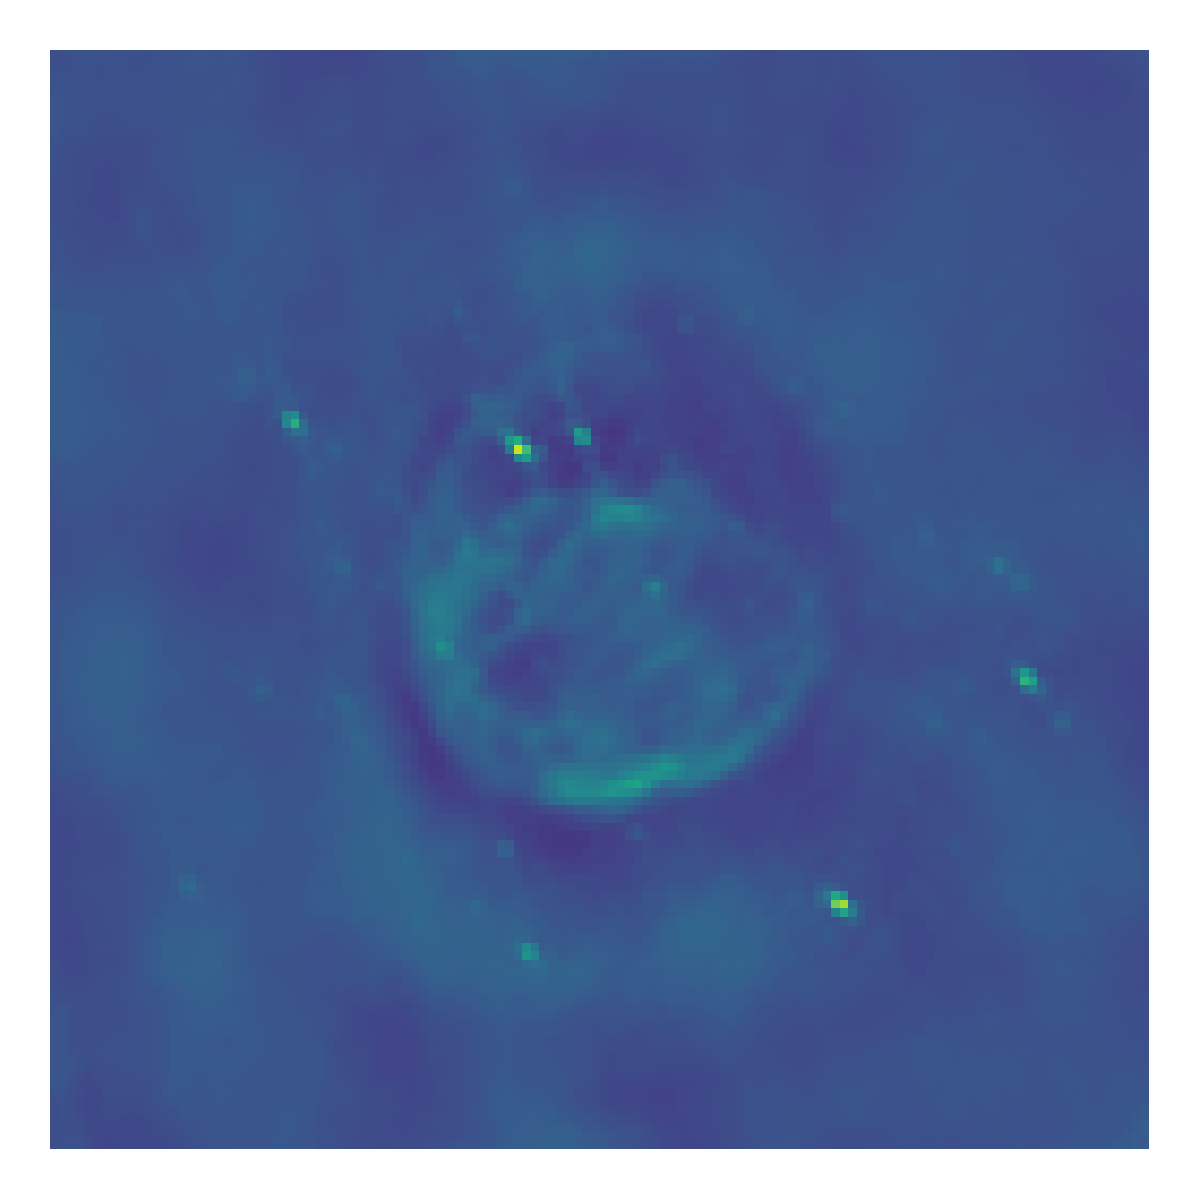
\includegraphics[width=\linewidth, trim={18px 19px 18px 18px}, clip]{./chapters/05.results/g55/starlets3_image.png}
	\end{subfigure}
	
	\rotatebox{90}{\makebox{\hspace{60pt}Model}}
	\begin{subfigure}[b]{0.3\linewidth}
		
\includegraphics[width=\linewidth, trim={18px 19px 18px 18px}, clip]{./chapters/05.results/g55/clean_model.png}
	\end{subfigure}
	\begin{subfigure}[b]{0.3\linewidth}
		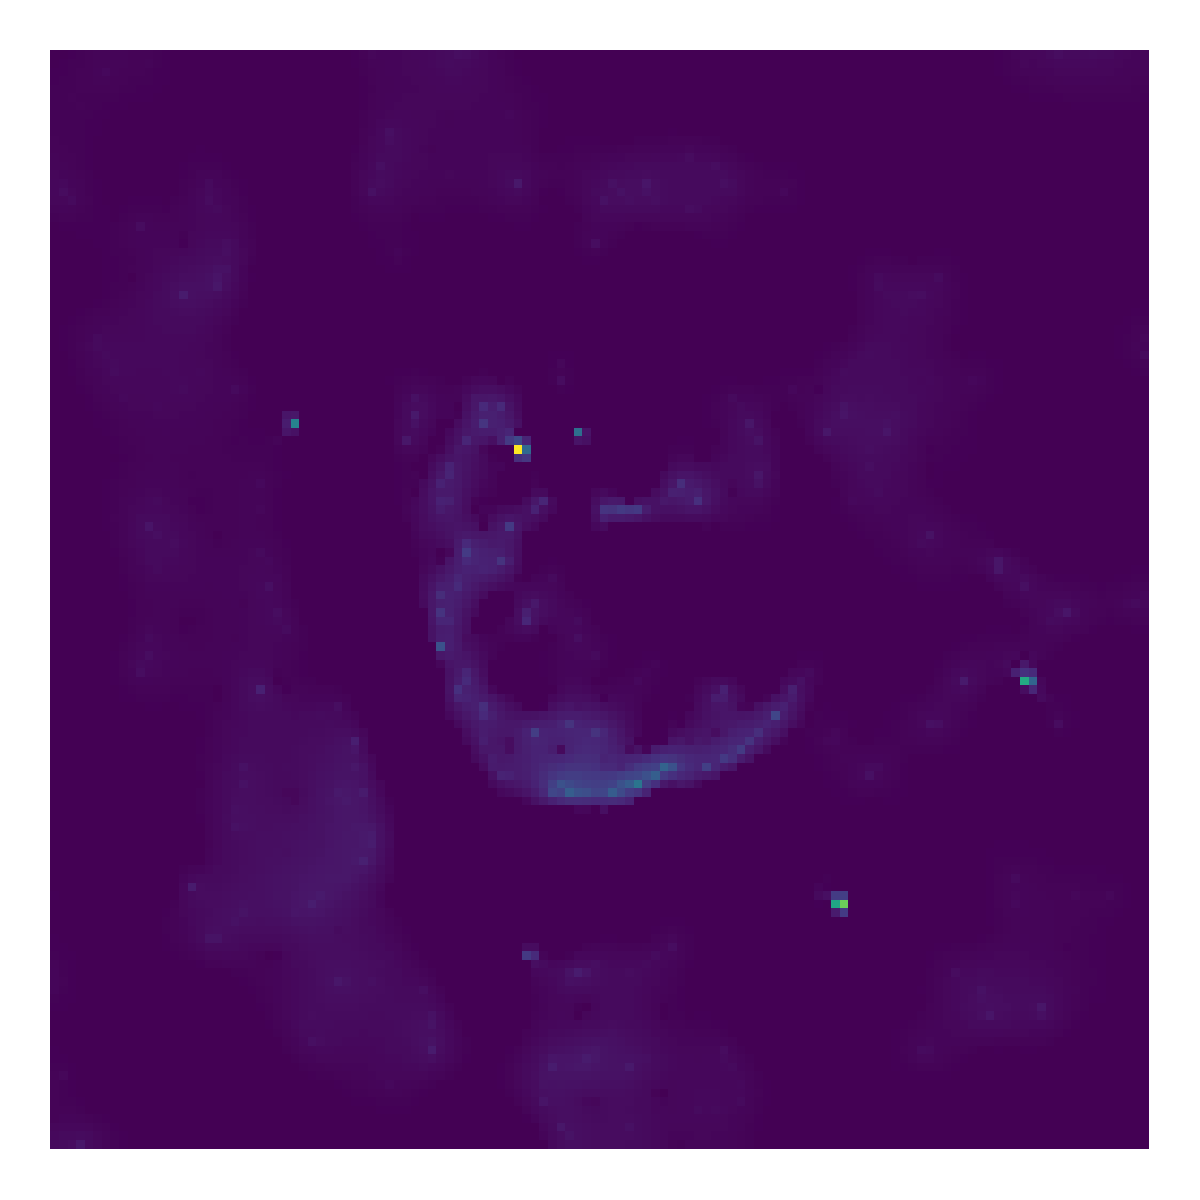
\includegraphics[width=\linewidth, trim={18px 19px 18px 18px}, clip]{./chapters/05.results/g55/starlets1_model.png}
	\end{subfigure}
	\begin{subfigure}[b]{0.3\linewidth}
		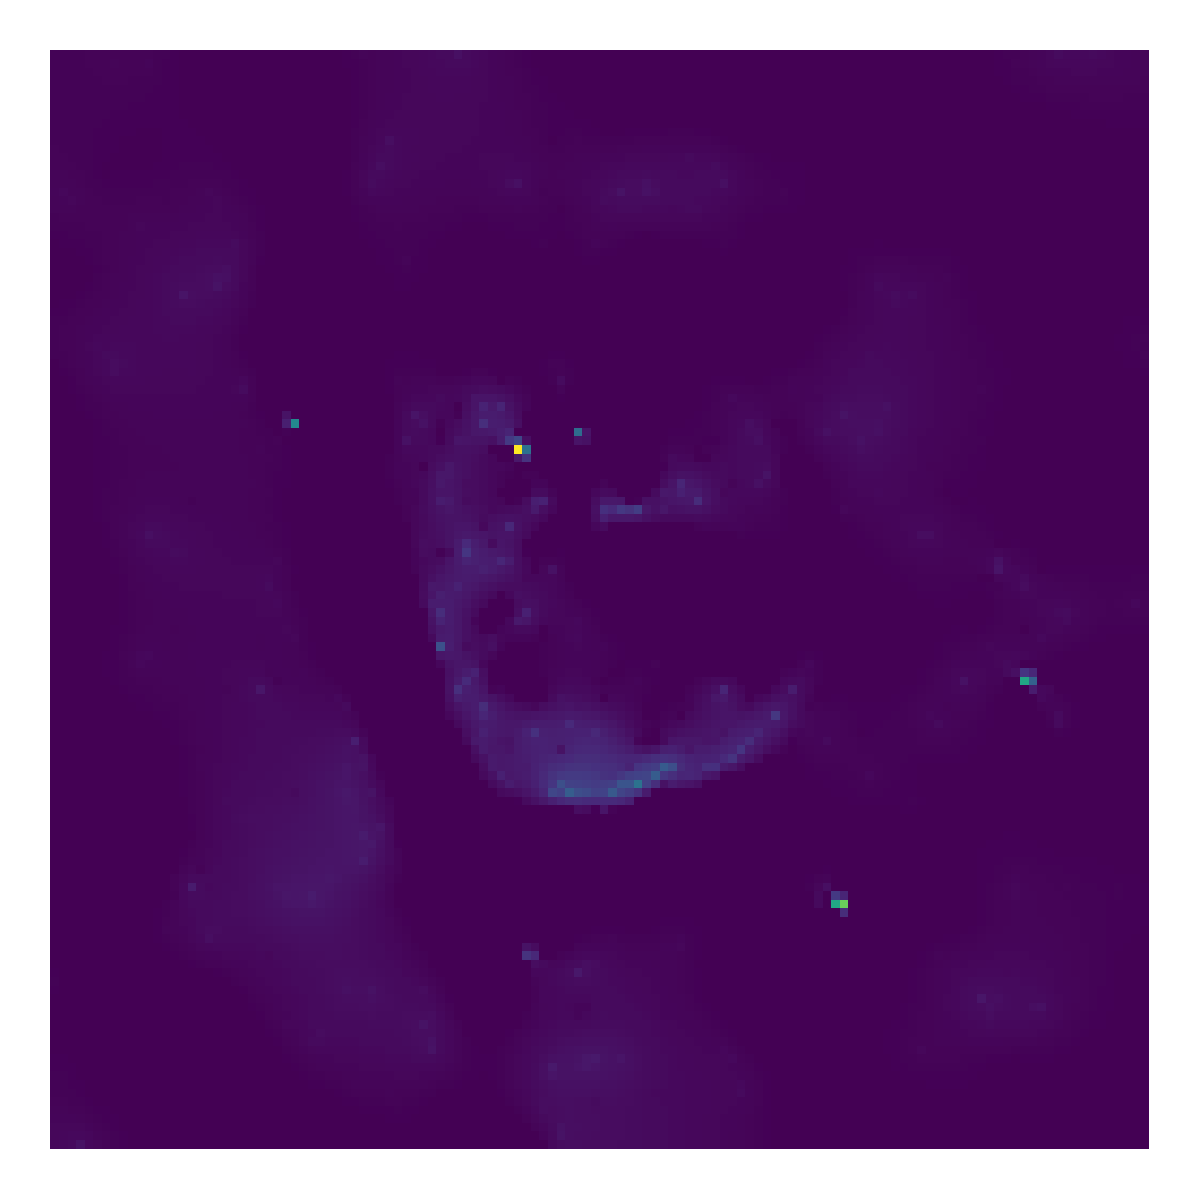
\includegraphics[width=\linewidth, trim={18px 19px 18px 18px}, clip]{./chapters/05.results/g55/starlets3_model.png}
	\end{subfigure}
	
	\rotatebox{90}{\makebox{\hspace{60pt}Residuals}}
	\begin{subfigure}[b]{0.3\linewidth}
		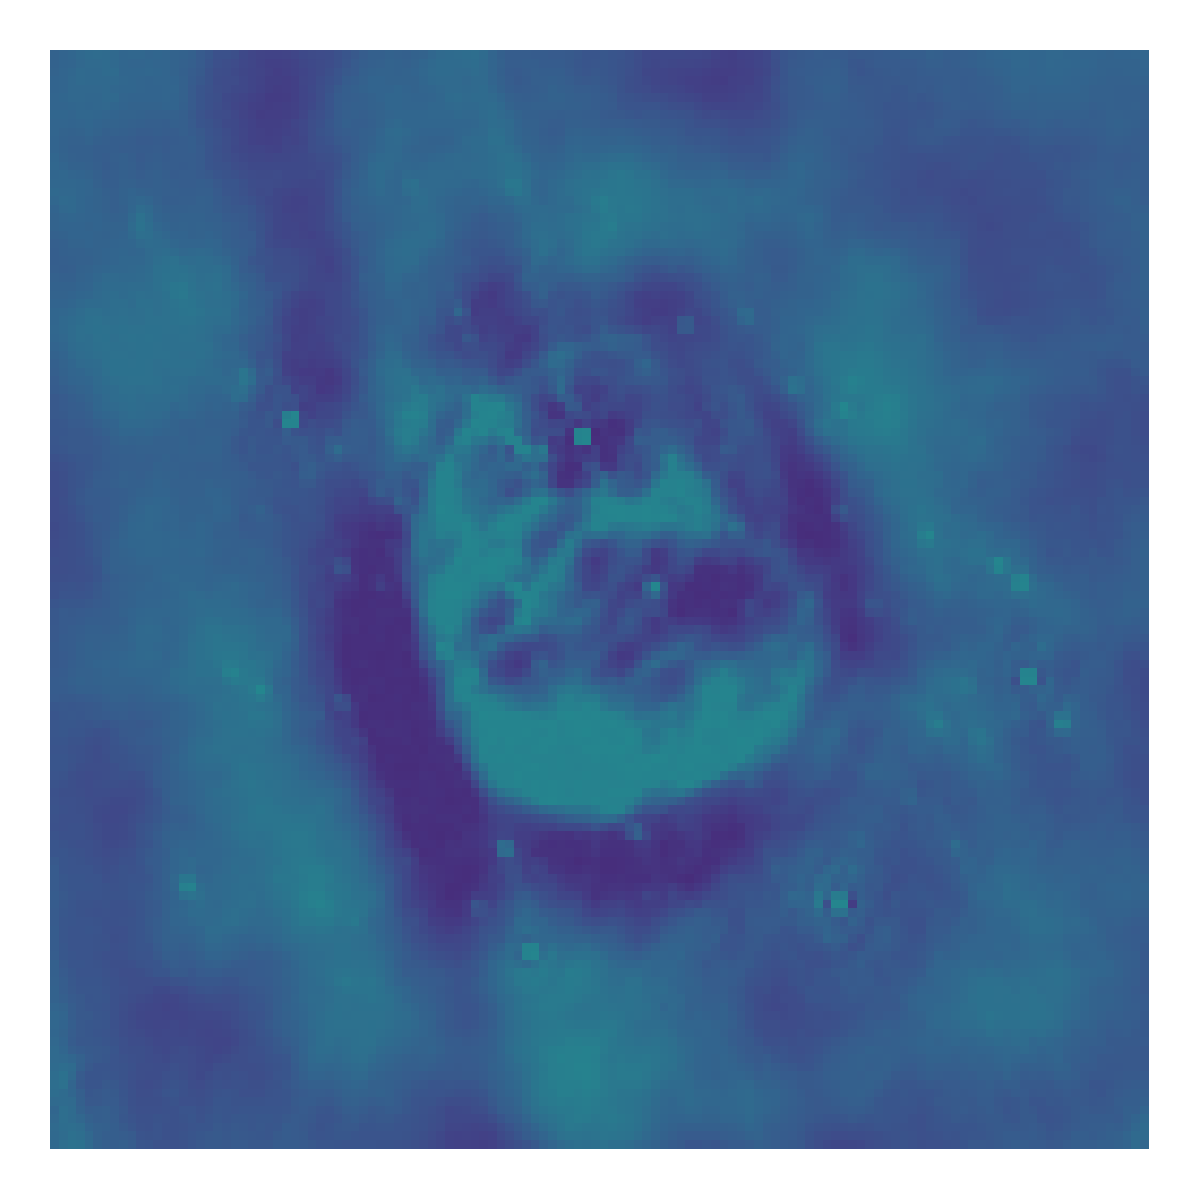
\includegraphics[width=\linewidth, trim={18px 19px 18px 18px}, clip]{./chapters/05.results/g55/clean_residual.png}
	\end{subfigure}
	\begin{subfigure}[b]{0.3\linewidth}
		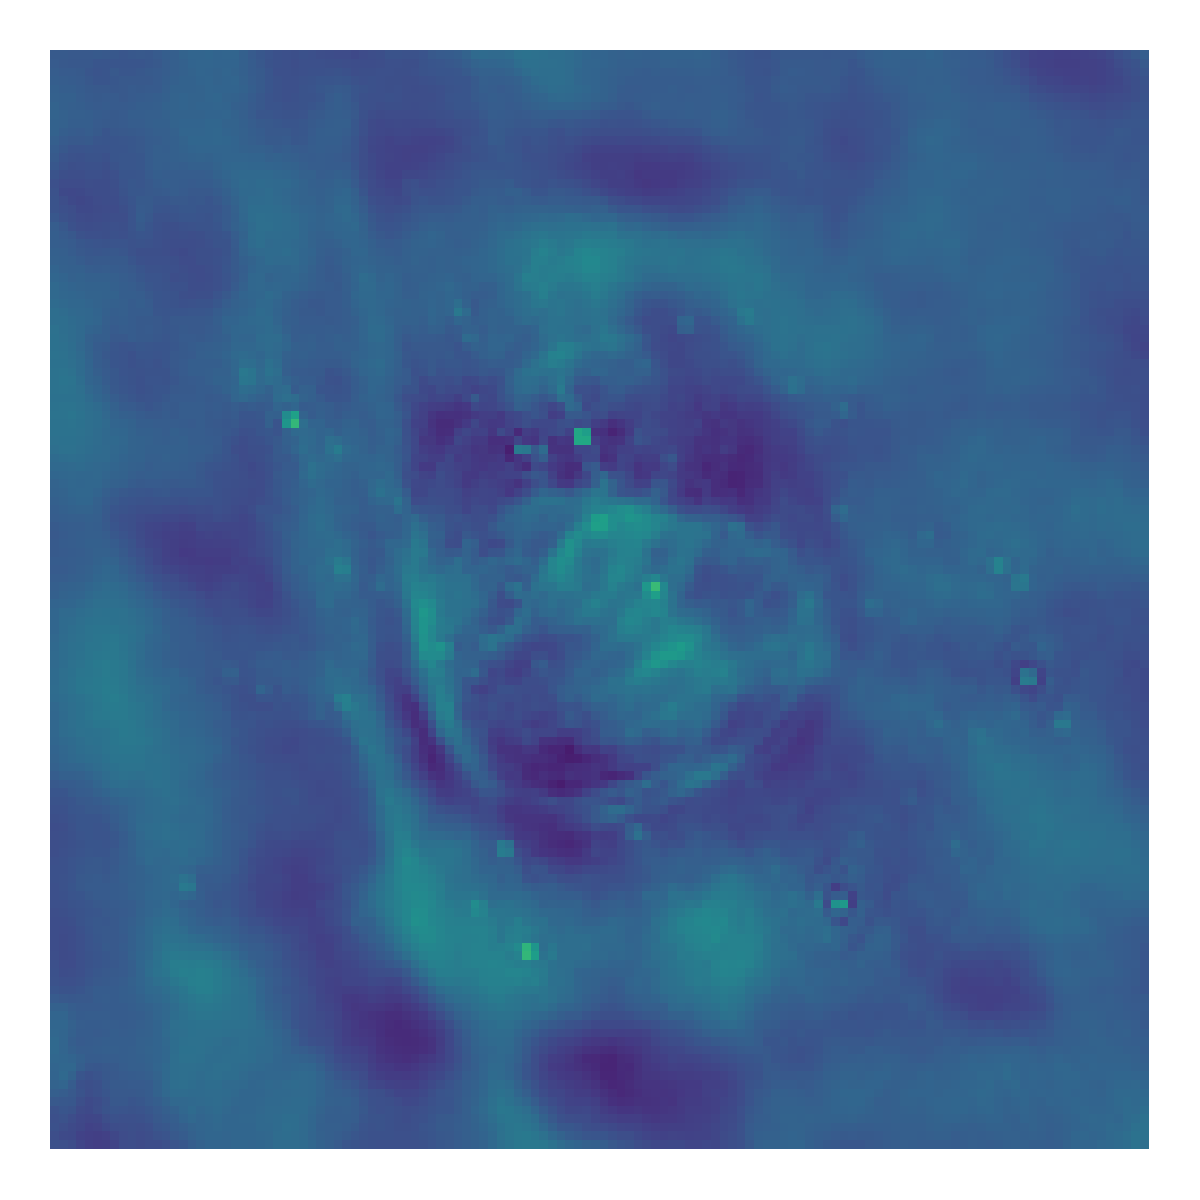
\includegraphics[width=\linewidth, trim={18px 19px 18px 18px}, clip]{./chapters/05.results/g55/starlets1_residual.png}
	\end{subfigure}
	\begin{subfigure}[b]{0.3\linewidth}
		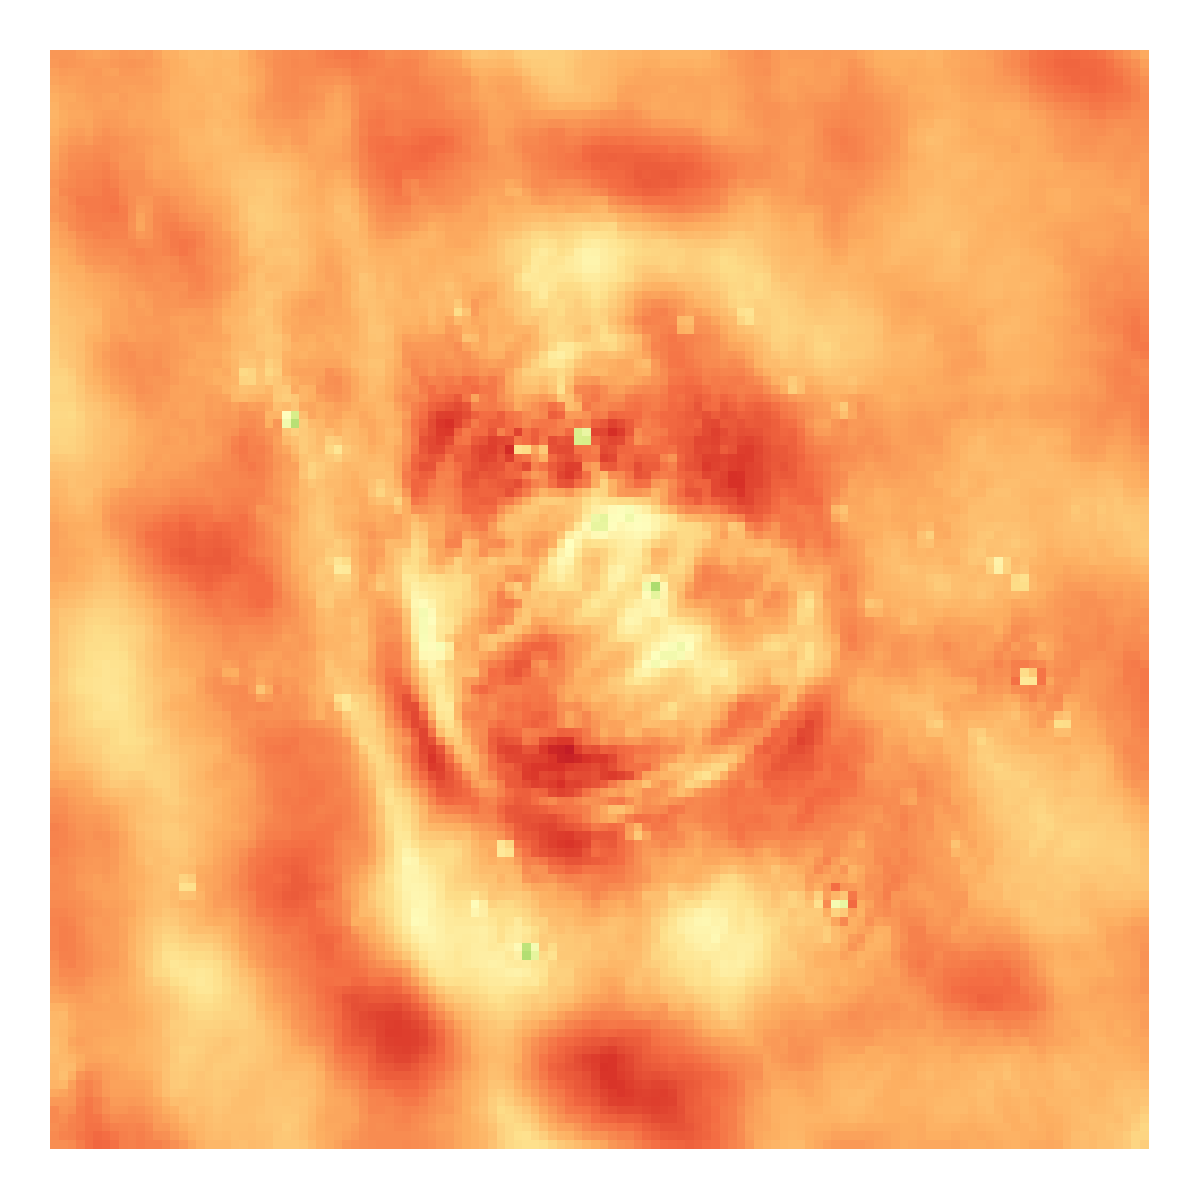
\includegraphics[width=\linewidth, trim={18px 19px 18px 18px}, clip]{./chapters/05.results/g55/starlets3_residual.png}
	\end{subfigure}
\end{figure}

starlets finds a lot of smaller point sources, but they do

plot with all stuff done

\subsection{Simple Priors}

pixels l1 norm

pixels l2 norm

Total Variation

Haar 

\subsection{Starlet Transform as Prior}

starlet decomposition

the cJ map as a smart thresholder

Runtime issues


last comparison, CLean, TV, starlet